\documentclass[
  paper=a4,
  fontsize=11pt,
  english,
  numbers=noenddot,
  parskip=half,
  cdgeometry=symmetric,
  cd=barcolor,
  % Remove this option and comment out the three font lines below to restore
  % the default TUD Open Sans body font.
  cdfont=false
]{tudscrartcl}

\usepackage[utf8]{inputenc}
\usepackage[T1]{fontenc}
\usepackage{babel}
\usepackage{microtype}
\usepackage{xspace}
\usepackage{graphicx}
\usepackage{xcolor}
\graphicspath{{assets/}}
\usepackage{etoolbox}
\makeatletter
\patchcmd{\tud@mainlogo@set}{\@tempa{TUD-black}}{\@tempa{assets/TUD-black}}{}{}
\patchcmd{\tud@mainlogo@set}{\@tempa{TUD-blue}}{\@tempa{assets/TUD-blue}}{}{}
\patchcmd{\tud@mainlogo@set}{\@tempa{TUD-white}}{\@tempa{assets/TUD-white}}{}{}
\makeatother
\usepackage{amsmath,amssymb}
% Palatino-style serif text and matching mathematics
\usepackage[nohelv]{newpxtext}
\usepackage{newpxmath}
\renewcommand{\sfdefault}{opensans-TLF} % Keep TUD Open Sans for headings
\usepackage{booktabs}
\usepackage{tabularx}
\usepackage{subcaption}
\captionsetup{font=small}
\captionsetup[subfigure]{font=small}
\usepackage{siunitx}
\usepackage[section]{placeins} % keep floats inside their section
\usepackage{csquotes}
\usepackage[
  backend=biber,
  style=numeric,
  sorting=none
]{biblatex}
\addbibresource{references.bib}
\usepackage[hidelinks]{hyperref}
\usepackage[capitalise,noabbrev,nameinlink]{cleveref}
\makeatletter
\DeclareRobustCommand\onedot{\futurelet\@let@token\@onedot}
\def\@onedot{\ifx\@let@token.\else.\null\fi\xspace}

\def\eg{\emph{e.g}\onedot}
\def\Eg{\emph{E.g}\onedot}
\def\ie{\emph{i.e}\onedot}
\def\Ie{\emph{I.e}\onedot}
\def\cf{\emph{cf.}\xspace}
\def\Cf{\emph{Cf.}\xspace}
\def\etc{\emph{etc}\onedot}
\def\vs{\emph{vs}\onedot}
\def\wrt{w.r.t\onedot}
\def\etal{\emph{et~al}\onedot}
\makeatother

\newcommand{\R}{\mathbb{R}}
\newcommand{\Z}{\mathbb{Z}}
\newcommand{\N}{\mathbb{N}}
\newcommand{\Q}{\mathbb{Q}}
\newcommand{\C}{\mathbb{C}}

% Information still to be filled in (printed in orange)
\DeclareRobustCommand{\todotext}[1]{\textcolor{orange}{[#1]}}
\newcommand{\todo}[1]{\texorpdfstring{\todotext{#1}}{[#1]}}

% Numbers and tables of the state-of-the-art comparison (Section 7) are generated from the
% result files by scripts/fidelity/paper_numbers.py; copy them with `make sync`.
% generated by scripts/fidelity/paper_numbers.py -- do not edit
\newcommand{\NFrames}{12}
\newcommand{\NlabTotal}{2{,}958}
\newcommand{\NlabMin}{102}
\newcommand{\NlabMax}{362}
\newcommand{\NFits}{80}
\newcommand{\NPairs}{80}
\newcommand{\RecallLoG}{94\%}
\newcommand{\FramesLoG}{12}
\newcommand{\RecallWS}{89\%}
\newcommand{\FramesWS}{12}
\newcommand{\RecallCP}{75\%}
\newcommand{\FramesCP}{12}
\newcommand{\RecallCPthree}{82\%}
\newcommand{\FramesCPthree}{12}
\newcommand{\JXLmax}{82--120$\times$}
\newcommand{\JXLworst}{91\%}
\newcommand{\FarRatio}{319--603$\times$}
\newcommand{\JtkMaxRatio}{603$\times$}
\newcommand{\PairsNLoG}{80}
\newcommand{\PairsJLoG}{33}
\newcommand{\PairsLLoG}{14}
\newcommand{\ModNLoG}{38}
\newcommand{\ModJLoG}{4}
\newcommand{\ModLLoG}{10}
\newcommand{\ModDiffLoG}{$+$1.2}
\newcommand{\FarDiffLoG}{$-$16.8}
\newcommand{\FarJLoG}{29 of 42}
\newcommand{\FarJtkLoG}{98--103\%}
\newcommand{\FarLuxLoG}{25--107\%}
\newcommand{\PairsNWS}{80}
\newcommand{\PairsJWS}{63}
\newcommand{\PairsLWS}{0}
\newcommand{\ModNWS}{38}
\newcommand{\ModJWS}{22}
\newcommand{\ModLWS}{0}
\newcommand{\ModDiffWS}{$-$4.2}
\newcommand{\FarDiffWS}{$-$19.8}
\newcommand{\FarJWS}{41 of 42}
\newcommand{\FarJtkWS}{96--100\%}
\newcommand{\FarLuxWS}{32--98\%}
\newcommand{\PairsNCP}{80}
\newcommand{\PairsJCP}{56}
\newcommand{\PairsLCP}{0}
\newcommand{\ModNCP}{38}
\newcommand{\ModJCP}{22}
\newcommand{\ModLCP}{0}
\newcommand{\ModDiffCP}{$-$9.4}
\newcommand{\FarDiffCP}{$-$23.5}
\newcommand{\FarJCP}{34 of 42}
\newcommand{\FarJtkCP}{84--101\%}
\newcommand{\FarLuxCP}{27--91\%}
\newcommand{\PairsNCPthree}{78}
\newcommand{\PairsJCPthree}{28}
\newcommand{\PairsLCPthree}{14}
\newcommand{\ModNCPthree}{36}
\newcommand{\ModJCPthree}{2}
\newcommand{\ModLCPthree}{14}
\newcommand{\ModDiffCPthree}{$+$3.7}
\newcommand{\FarDiffCPthree}{$-$18.7}
\newcommand{\FarJCPthree}{26 of 42}
\newcommand{\FarJtkCPthree}{102--116\%}
\newcommand{\FarLuxCPthree}{29--118\%}
\newcommand{\PSNRjtkWins}{80 of 80}
\newcommand{\FrModPSNR}{$-$2.4}
\newcommand{\FrModPSNRCI}{$-$2.7 to $-$2.1}
\newcommand{\FrModPSNRPos}{0}
\newcommand{\FrModPSNRNeg}{12}
\newcommand{\FrFarPSNR}{$-$1.4}
\newcommand{\FrFarPSNRCI}{$-$1.6 to $-$1.3}
\newcommand{\FrFarPSNRPos}{0}
\newcommand{\FrFarPSNRNeg}{12}
\newcommand{\FrModLoG}{$+$1.3}
\newcommand{\FrModLoGCI}{$+$0.0 to $+$2.7}
\newcommand{\FrModLoGPos}{8}
\newcommand{\FrModLoGNeg}{4}
\newcommand{\FrModLoGP}{0.110}
\newcommand{\FrModLoGEOne}{$+$0.3}
\newcommand{\FrModLoGETwo}{$+$2.4}
\newcommand{\FrFarLoG}{$-$16.6}
\newcommand{\FrFarLoGCI}{$-$23.0 to $-$10.2}
\newcommand{\FrFarLoGPos}{1}
\newcommand{\FrFarLoGNeg}{11}
\newcommand{\FrFarLoGP}{0.004}
\newcommand{\FrFarLoGEOne}{$-$17.6}
\newcommand{\FrFarLoGETwo}{$-$15.5}
\newcommand{\FrModWS}{$-$4.0}
\newcommand{\FrModWSCI}{$-$5.3 to $-$2.7}
\newcommand{\FrModWSPos}{0}
\newcommand{\FrModWSNeg}{12}
\newcommand{\FrModWSP}{0.004}
\newcommand{\FrModWSEOne}{$-$2.1}
\newcommand{\FrModWSETwo}{$-$5.9}
\newcommand{\FrFarWS}{$-$19.3}
\newcommand{\FrFarWSCI}{$-$23.8 to $-$15.0}
\newcommand{\FrFarWSPos}{0}
\newcommand{\FrFarWSNeg}{12}
\newcommand{\FrFarWSP}{0.004}
\newcommand{\FrFarWSEOne}{$-$19.0}
\newcommand{\FrFarWSETwo}{$-$19.6}
\newcommand{\FrModCP}{$-$9.4}
\newcommand{\FrModCPCI}{$-$11.4 to $-$7.3}
\newcommand{\FrModCPPos}{0}
\newcommand{\FrModCPNeg}{12}
\newcommand{\FrModCPP}{0.004}
\newcommand{\FrModCPEOne}{$-$12.3}
\newcommand{\FrModCPETwo}{$-$6.5}
\newcommand{\FrFarCP}{$-$23.2}
\newcommand{\FrFarCPCI}{$-$28.0 to $-$18.3}
\newcommand{\FrFarCPPos}{0}
\newcommand{\FrFarCPNeg}{12}
\newcommand{\FrFarCPP}{0.004}
\newcommand{\FrFarCPEOne}{$-$29.0}
\newcommand{\FrFarCPETwo}{$-$17.5}
\newcommand{\FrModCPthree}{$+$3.5}
\newcommand{\FrModCPthreeCI}{$+$1.8 to $+$5.5}
\newcommand{\FrModCPthreePos}{10}
\newcommand{\FrModCPthreeNeg}{2}
\newcommand{\FrModCPthreeP}{0.010}
\newcommand{\FrModCPthreeEOne}{$+$1.0}
\newcommand{\FrModCPthreeETwo}{$+$6.1}
\newcommand{\FrFarCPthree}{$-$18.2}
\newcommand{\FrFarCPthreeCI}{$-$23.8 to $-$12.8}
\newcommand{\FrFarCPthreePos}{0}
\newcommand{\FrFarCPthreeNeg}{12}
\newcommand{\FrFarCPthreeP}{0.004}
\newcommand{\FrFarCPthreeEOne}{$-$20.3}
\newcommand{\FrFarCPthreeETwo}{$-$16.0}
\newcommand{\FrN}{12}
\newcommand{\FrFarNeg}{11--12}
\newcommand{\DPSNR}{1.0--6.8\,dB}
\newcommand{\EarlyAdvPts}{8--11}
\newcommand{\EarlyAdvRatio}{159--537$\times$}
\newcommand{\Kstar}{64{,}000}
\newcommand{\KstarCalFrames}{4}
\newcommand{\KstarFrames}{4}
\newcommand{\KstarRatio}{25--30$\times$}
\newcommand{\KstarLoG}{101--103\%}
\newcommand{\KstarWS}{96--100\%}
\newcommand{\KstarCP}{89--98\%}
\newcommand{\KstarCPthree}{102--105\%}
\newcommand{\KstarJtk}{99--102\%}
\newcommand{\GapWS}{$+$0 to $+$5}
\newcommand{\GapFramesWS}{10}
\newcommand{\LuxMidWS}{93--99\%}
\newcommand{\GapCP}{$+$4 to $+$15}
\newcommand{\GapFramesCP}{10}
\newcommand{\LuxMidCP}{82--94\%}
\newcommand{\GapCPthree}{$-$18 to $-$4}
\newcommand{\GapFramesCPthree}{10}
\newcommand{\LuxMidCPthree}{104--118\%}
\newcommand{\LuxMidLoG}{98--106\%}
\newcommand{\RuleGapBigWS}{1 of 12}
\newcommand{\RuleGapSmallWS}{11 of 12}
\newcommand{\RuleGapBigCPthree}{0 of 12}
\newcommand{\RuleGapSmallCPthree}{12 of 12}
\newcommand{\RuleGapBigCP}{11 of 12}
\newcommand{\RuleGapSmallCP}{1 of 12}
\newcommand{\RulePsnrOK}{4 of 8}
\newcommand{\CPwobble}{8}
\newcommand{\RepLoG}{2.1}
\newcommand{\RepWS}{3.5}
\newcommand{\RepCP}{3.7}
\newcommand{\CliffBelow}{2.5}
\newcommand{\CliffOne}{64--92\%}
\newcommand{\CrossRange}{1.1--3.1}
\newcommand{\LuxPSNRrange}{19.0--23.2\,dB}
\newcommand{\LuxPSNRspan}{2.6\,dB}
\newcommand{\FitA}{17--46\,min}
\newcommand{\FitH}{5--40\,min}
\newcommand{\SurvRho}{0.66}
\newcommand{\SurvN}{80}


% Document metadata
\faculty{Faculty of Computer Science}
\institute{}
\chair{Chair of Machine Learning for Spatial Understanding}
\subject{Team Project Report}
\title{Gaussian Blobs for 3D Fluorescence Microscopy}
\subtitle{Fitting light-sheet volumes with 3D Gaussians,\\and testing whether the nuclei survive}
% TODO: Akim's matriculation number (\todo cannot be used here)
\author{Syed Muhammad Asad (5301662)\and Akim Al-Makhdar ([Matr.-Nr.])}
\date{Supervisor: Prof.\ Dr.\ Martin Weigert\\[0.5ex]\today}

\begin{document}

\maketitle

\begin{abstract}
\noindent Light-sheet microscopes record developing embryos as terabytes of 3D volumes. One
proposed remedy is to store each volume as a set of 3D Gaussian blobs (``splats''), which is
compact and renders quickly; such representations are judged almost only by PSNR. This
project asked two questions. Can a Gaussian fit be made to keep the cell nuclei that
biologists measure? And does the state-of-the-art Gaussian compressor keep them as well as a
standard codec at the same file size? Starting from a synthetic phantom with a known answer,
we tested changes one at a time on real \emph{Tribolium} data: where blobs start, their shape,
densification, a budget derived from the cell count, the position learning rate, and a size
cap for nucleus blobs. Starting one blob on every detected nucleus raised the share of nuclei
found after fitting from 52\% to 71\%, and the cap recovered 6 of 31 faint nuclei at no
measurable PSNR cost; on 29 hand-labelled \emph{Drosophila} nuclei, however, a classical blob
filter put more of them into the top 100 detections than any fit. At identical bytes on 12 \emph{C.~elegans} frames with
\NlabTotal{} labelled nuclei, JPEG2000 had higher PSNR than the Luxar Gaussian compressor on
every frame, yet the number of nuclei found depended on the detector: below
\SI{300}{\times} compression, 3D Cellpose found \FrModCPthree{} percentage points more nuclei
in splat reconstructions, while a watershed and 2D Cellpose found \FrModWS{} and \FrModCP{}
points fewer. Beyond \SI{300}{\times}, at fewer than about three splats per nucleus, splats
lost 17--23 points for every detector. PSNR alone cannot decide which storage format is safe for
a given analysis.
\end{abstract}

\clearpage
\tableofcontents
\clearpage

% =====================================================================
\section{Introduction}\label{sec:intro}
% =====================================================================

\subsection{The problem}

Light-sheet microscopy images living embryos layer by layer, quickly and with little light
damage, and records them as time series of 3D volumes. One frame of our \emph{Tribolium}
recording has 37~million voxels; one \emph{C.~elegans} recording of the Cell Tracking
Challenge~\cite{maska2023cell} has 195 frames and takes about \SI{2.5}{GB} even at 8~bit, and
real experiments run for hours and produce terabytes. Such data are hard to store, share and
look at.

3D Gaussian splatting~\cite{kerbl2023gaussian} offers a different way to store a volume: as a
sum of a few thousand soft, stretched 3D blobs, each described by 11 numbers. The
representation is continuous, compact and fast to draw on a graphics card. It has recently been
adapted to microscopy~\cite{royer2026luxar,gaussianpile2026}, to medical volumes for compact
storage~\cite{gstoken2026,martin2026fixedbudget} and to CT
reconstruction~\cite{zha2024r2gaussian,li2025threedgr}. All of these are evaluated by global
image similarity (PSNR, SSIM). For biologists the relevant question is different: after
compression, does the analysis they run still find the cells? A nucleus is a small, often faint
peak, and a smooth fit can lose it while the PSNR barely changes.

\subsection{What we set out to solve, and by how much}

The project addressed two concrete questions:
\begin{enumerate}
  \item \textbf{Fitting.} Starting from the simplest working setup, which changes make a
        Gaussian fit keep the nuclei, and how much does each change help?
  \item \textbf{State of the art.} At exactly the same number of bytes on disk, does the
        strongest existing Gaussian compressor (Luxar~\cite{royer2026luxar}) keep as many
        nuclei as a standard codec (JPEG2000), as judged by the detectors biologists use?
\end{enumerate}
\Cref{tab:summary} summarises the answers. In short, our fitting changes made Gaussian fits
keep nuclei much more reliably than the naive setup, but a classical blob filter applied to the
raw image ranks nuclei better in the top 100 and as well in the top 200; and at matched file size the state-of-the-art splats are
neither uniformly better nor uniformly worse than JPEG2000: the winner depends on the detector,
which PSNR cannot reveal.

\begin{table}[tb]
  \centering\small
  \begin{tabularx}{\linewidth}{@{}>{\raggedright\arraybackslash}p{3.6cm}>{\raggedright\arraybackslash}X>{\raggedright\arraybackslash}p{4.4cm}@{}}
    \toprule
    Question & Answer & By how much \\
    \midrule
    Do more careful fits keep more nuclei? (our fitter, \emph{Tribolium})
      & Yes: start one blob per nucleus, cap the size of nucleus blobs
      & nuclei found 52\% $\to$ 71\%; faint nuclei 13 $\to$ 19 of 31; PSNR unchanged \\
    Is the fit better than the raw image for finding labelled nuclei? (\emph{Drosophila}, 29 labels)
      & Better than brightness ranking; worse than a blob filter in the top 100, level in the top 200
      & top-100 hits: fit 14, raw brightness 10, LoG filter 16--18 \\
    Do state-of-the-art splats keep more nuclei than JPEG2000 at the same bytes? (\emph{C.~elegans}, 12 frames)
      & Depends on the detector below \SI{300}{\times}; never beyond
      & 3D Cellpose \FrModCPthree, watershed \FrModWS, 2D Cellpose \FrModCP{} points; beyond
        \SI{300}{\times} \FrFarLoG{} to \FrFarCP{} points \\
    Does PSNR predict this? & No: it prefers JPEG2000 everywhere & JPEG2000 higher on 12/12 frames and 80/80 pairs \\
    Where do splats break? (\emph{C.~elegans}, LoG) & Below about three splats per nucleus & nuclei kept crosses 90\% at \CrossRange{} splats per nucleus, on 12/12 frames \\
    \bottomrule
  \end{tabularx}
  \caption{Summary of outcomes. ``Points'' are percentage points of \emph{nuclei kept} (nuclei
  found after compression divided by nuclei found in the raw volume by the same detector);
  negative means JPEG2000 kept more. Details in \cref{sec:steps,sec:validation,sec:sota}.}
  \label{tab:summary}
\end{table}

\subsection{Division of work}

The project was carried out by two students. \textbf{Akim Al-Makhdar} built the first fitting pipeline
and ran the exploratory experiment archive (399 fits in 57 experiments): the phantom
experiments on starting positions, the sweep over blob shapes and budgets on real data,
densification, and the cell-count budget (Steps~1--4 in \cref{sec:steps}). \textbf{Syed
Muhammad Asad} re-analysed this archive and built the evaluation framework (physical units,
object-level matching, regression tests), ran the controlled experiments on repeats, seeding,
learning rate and size cap (Steps~5--8), the check against human labels (\cref{sec:validation}),
and the state-of-the-art comparison (\cref{sec:sota}). The phantom (Step~0) and the
representation were shared work.

\subsection{Outline}

\Cref{sec:related} places the work in context, \cref{sec:data} describes the data and
\cref{sec:repr} the representation, fitting and evaluation. \Cref{sec:steps} goes from a
phantom to the final fitting recipe, one change at a time, stating for each change what was
changed, why it should help, and what it did. \Cref{sec:validation} checks whether the fits
behave as expected and compares them with naive baselines, and \cref{sec:sota} compares
Gaussian compression with standard codecs at matched file size. \Cref{sec:discussion}
discusses limitations and the next steps. A glossary of technical terms is in
\cref{app:glossary}.

% =====================================================================
\section{Related work}\label{sec:related}
% =====================================================================

\paragraph{Gaussians for nuclei.} Gaussian mixtures have long been used to segment and track
nuclei in light-sheet data, most prominently TGMM~\cite{amat2014fast}, which also limits the
covariance of each Gaussian. Representing nuclei as Gaussians, or capping their size, is
therefore not new on its own; our question concerns Gaussians as a \emph{storage format}.

\paragraph{Gaussian volume representations.} 3D Gaussian splatting~\cite{kerbl2023gaussian}
renders opaque scenes for a camera by alpha-compositing. It has been adapted to tomographic
reconstruction~\cite{zha2024r2gaussian,li2025threedgr}, to slice-to-volume MRI with closed-form
point-spread functions~\cite{dannecker2026fast}, and to the compression of microscopy and
medical volumes~\cite{royer2026luxar,gaussianpile2026,gstoken2026,martin2026fixedbudget}. Luxar
fits splats to large microscopy volumes in minutes on one GPU and chooses the number of splats
by a self-supervised held-out PSNR~\cite{batson2019noise2self}; its authors describe the fits
as intended for visualisation rather than quantitative analysis. All of these works report
global image fidelity.

\paragraph{Compression of microscopy data.} Biologists mostly store raw data losslessly. B3D
compresses light-sheet data in real time, losslessly or with errors bounded by the camera
noise~\cite{balazs2017b3d}, and the adaptive particle representation stores a volume as
particles whose density follows the local image resolution~\cite{cheeseman2018adaptive}. Lossy
image codecs such as JPEG2000~\cite{taubman2002jpeg2000} and JPEG-XL~\cite{alakuijala2019jpegxl}
are the natural baselines at matched size. In radiology, lossy compression is judged by whether
lesions remain detectable, not by PSNR~\cite{koff2006overview}; Gaussian volume compression has
not yet been held to that standard.

\paragraph{Detection and labels.} We use Cell Tracking Challenge
annotations~\cite{ulman2017objective,maska2023cell}, a scale-normalised Laplacian of Gaussian
(LoG)~\cite{lindeberg1998feature}, a distance-transform watershed, and
Cellpose~\cite{stringer2021cellpose}.

% =====================================================================
\section{Data}\label{sec:data}
% =====================================================================

We used three real light-sheet recordings of developing embryos and one synthetic phantom
(\cref{tab:data,fig:data}). The depth step is much larger than the pixel size, so nuclei look
stretched along $z$; every spatial setting in this work is therefore given in micrometres and
converted per axis, never in voxels.

\begin{table}[tb]
  \centering\small
  \begin{tabularx}{\linewidth}{@{}l>{\raggedright\arraybackslash}p{2.6cm}>{\raggedright\arraybackslash}p{2.6cm}>{\raggedright\arraybackslash}X@{}}
    \toprule
    Dataset & Voxel size $z{\times}y{\times}x$ (\si{\micro\meter}) & Reference nuclei & Use \\
    \midrule
    Synthetic phantom & isotropic & exact (generated) & Step~0: does the fitting code recover a known answer? \\
    \emph{Tribolium castaneum} (frame i000022) & $3.0\times0.69\times0.69$ & detector-derived &
      Development: $64\times128\times128$ crops and the whole volume ($71\times1024\times512$) \\
    \emph{Drosophila}, Fluo-N3DL-DRO (CTC) & $2.03\times0.406\times0.406$ & 189 human-labelled tracks &
      Validation against human labels; a selected subset is labelled, so precision is not interpretable \\
    \emph{C.~elegans}, Fluo-N3DH-CE (CTC) & $1.0\times0.09\times0.09$ & every nucleus labelled &
      State-of-the-art comparison: 12 frames of two embryos, \NlabTotal{} nuclei \\
    \bottomrule
  \end{tabularx}
  \caption{Datasets. CTC: Cell Tracking Challenge~\cite{maska2023cell}. Detector-derived
  references are positions found by a peak detector; human labels are positions marked by
  experts and are the only non-circular reference.}
  \label{tab:data}
\end{table}

\begin{figure}[tb]
  \centering
  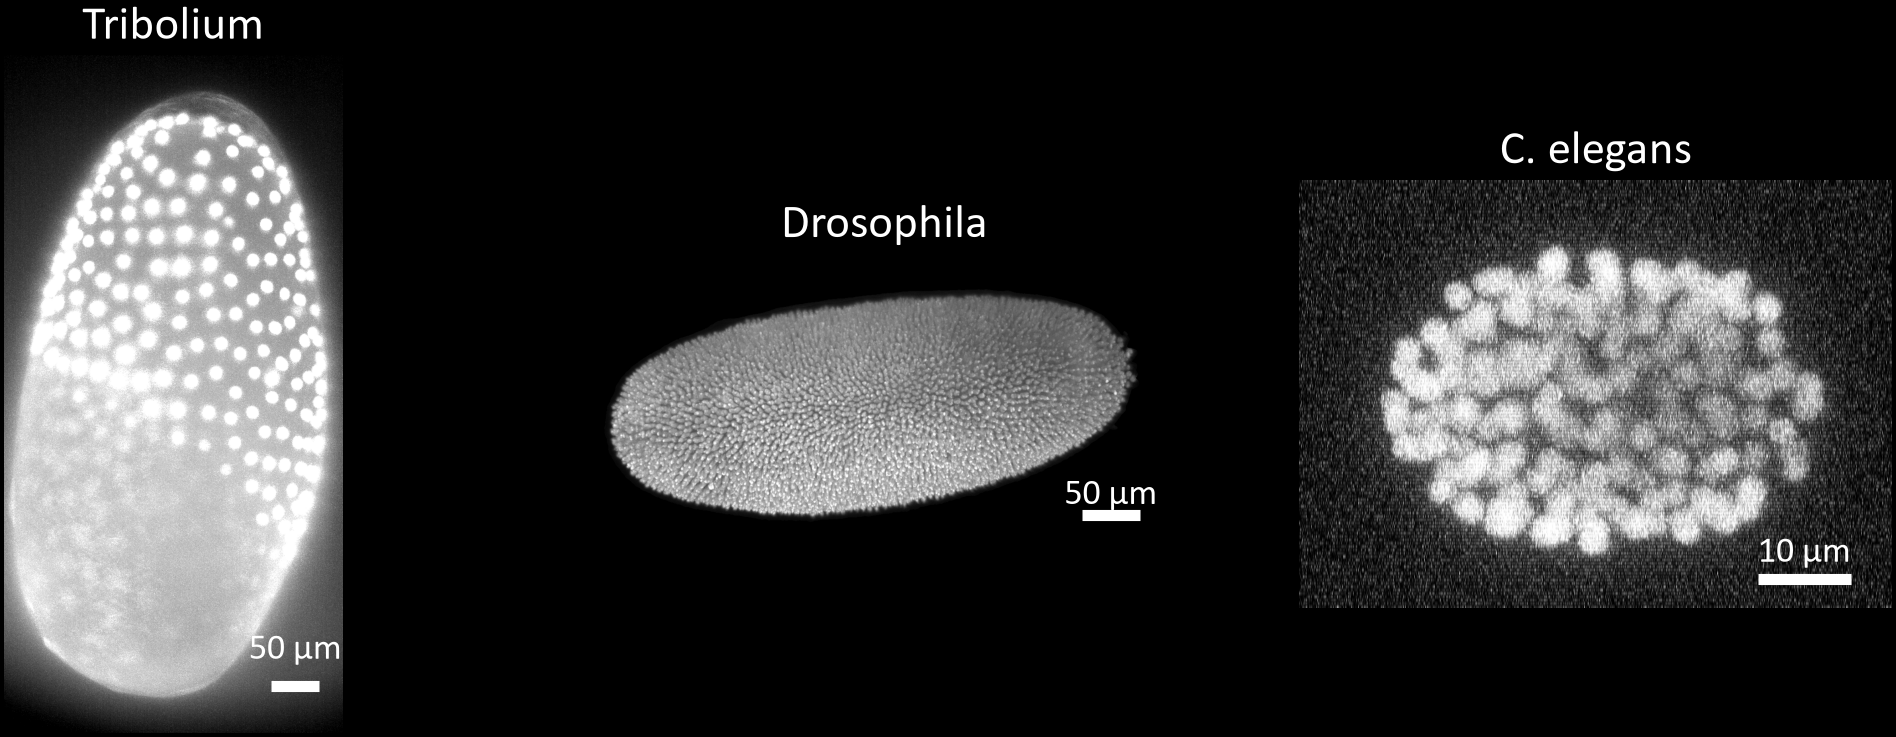
\includegraphics[width=\linewidth]{figs/data_three.png}
  \caption{The three real recordings, shown as maximum-intensity projections (for each line of
  sight the brightest voxel). Nuclei are fluorescently labelled and appear as bright blobs.}
  \label{fig:data}
\end{figure}

For the state-of-the-art comparison we used six frames of each of the two \emph{C.~elegans}
embryos (sequence~01: t110, t130, t150, t170, t185, t194; sequence~02: t110, t130, t150, t165,
t180, t185), with \NlabMin--\NlabMax{} labelled nuclei per frame. Four frames were chosen
first; eight were added later under rules fixed before the data were analysed
(\cref{app:rules}). Embryo~1 t100, whose early nuclei are larger, is reported separately.
Nuclei measure about $D=\SI{3.6}{\micro\meter}$, and all spatial parameters of that study are
fixed multiples of $D$.

% =====================================================================
\section{Representation, fitting and evaluation}\label{sec:repr}
% =====================================================================

\subsection{A volume as a sum of Gaussians}

A volume $I(\mathbf{x})$ is approximated by $K$ Gaussian blobs,
\begin{equation}
  \hat I(\mathbf{x}) = \sum_{k=1}^{K} a_k \exp\!\Big(-\tfrac12(\mathbf{x}-\boldsymbol\mu_k)^\top
  \Sigma_k^{-1}(\mathbf{x}-\boldsymbol\mu_k)\Big),\qquad
  \Sigma_k = R(\mathbf{q}_k)\,S_k S_k^\top R(\mathbf{q}_k)^\top,
  \label{eq:model}
\end{equation}
with position $\boldsymbol\mu_k\in\R^3$, scales $S_k=\operatorname{diag}(s_{k,x},s_{k,y},s_{k,z})$
stored as logarithms, rotation $R$ given by a unit quaternion $\mathbf{q}_k$, and amplitude
$a_k$. Each blob stores 11 numbers (3 + 3 + 4 + 1) and has 10 degrees of freedom, because the
quaternion is normalised. Simpler variants fix the rotation (\emph{axis-aligned} or
\emph{stretched}), tie the three scales (\emph{isotropic} or \emph{round}), or fix the scale
altogether. \Cref{fig:repr} shows a real crop and its fit with 250 blobs: 2{,}750 stored
numbers instead of about one million voxels. This is a count of numbers, not a measured file
size; file sizes are compared in \cref{sec:sota}.

\begin{figure}[tb]
  \centering
  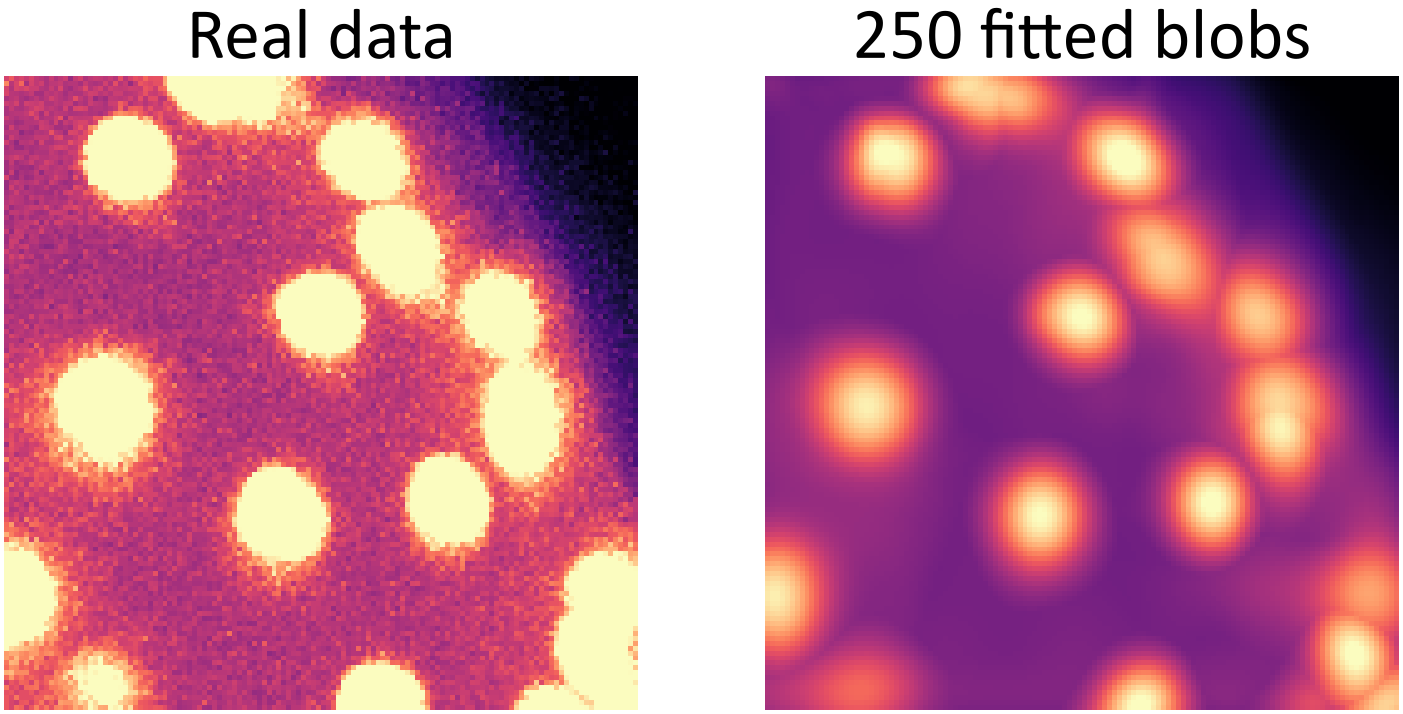
\includegraphics[width=0.8\linewidth]{figs/real_vs_fit.png}
  \caption{A $64\times128\times128$ \emph{Tribolium} crop (left) and its reconstruction from
  250 fitted Gaussians (right), maximum projections along $z$, each scaled to its own
  1st--99.5th percentile. Nuclei are kept as smooth blobs; the fine texture is smoothed away.}
  \label{fig:repr}
\end{figure}

\subsection{Fitting}

The fit evaluates \cref{eq:model} directly at voxel centres and minimises the squared error to
the data with Adam~\cite{kingma2015adam}, typically for 3{,}000 iterations. Each iteration
uses a random batch of voxels: 70\% drawn in proportion to intensity and 30\% uniformly,
without importance correction, so the effective objective weights bright voxels more than
plain squared error. Ten percent of voxels are held out for validation. Held-out PSNR measures
interpolation within a volume, not generalisation, because the initialisation sees the whole
volume. We do \emph{not} use the alpha-compositing renderer of 3D Gaussian splatting, for the
reason given in Step~0.

\subsection{Evaluation}\label{sec:eval}

\paragraph{Image quality.} The peak signal-to-noise ratio (PSNR, in dB) between reconstruction
and data; higher is better, and $+3$\,dB roughly halves the squared error.

\paragraph{Object fidelity.} A detector is run on the reconstruction and its detections are
matched one-to-one to reference nuclei within a radius. Three rules turned out to be essential,
each learned from a bug (\cref{app:bugs}):
\begin{itemize}
  \item \textbf{Physical units.} Detection windows, smoothing and matching radii are set in
        micrometres. A 13-voxel cubic window spans \SI{26}{\micro\meter} in $z$ but
        \SI{5.3}{\micro\meter} in $xy$ on \emph{Drosophila}; with it the detector recovered 5
        of 29 labelled nuclei from the raw volume, with a physical window 22 of 29.
  \item \textbf{Maximum-cardinality matching.} Minimum-cost assignment followed by a radius
        filter can drop valid matches; out-of-radius pairs are now penalised so that the number
        of matches is maximised first.
  \item \textbf{Matched budgets.} Recall grows with the number of detections, so methods are
        compared at the same number of detections (top~$N$).
\end{itemize}
We report \emph{recall} (share of reference nuclei found), \emph{F1} (harmonic mean of recall
and precision) and, for compression, \emph{nuclei kept}: nuclei found after compression divided
by nuclei found in the raw volume by the same detector. A value of 1 means that the same number
of labelled nuclei was found, not necessarily the same individual nuclei. A suite of 24
regression tests pins
every evaluation bug we found.

% =====================================================================
\section{From a simple setup to the final recipe}\label{sec:steps}
% =====================================================================

We started from the simplest setup that can be checked exactly, a synthetic phantom, and then
tested one change at a time on real data, each in its own comparison under the settings stated
there. For each change we state what was changed, why it was expected to help, and what it
did. Steps~1--4 are Akim's experiments, Steps~5--8 ours.

\subsection{Step 0: a phantom with a known answer}

\textbf{Setup.} A $64\times128\times128$ volume made of 50 Gaussian blobs of random size,
orientation and brightness, fitted with 2{,}000 Gaussians for 3{,}000 iterations by comparing
the Gaussian sum with the volume at every voxel. \textbf{Why.} The phantom is itself a Gaussian
sum, so correct code must recover it almost exactly. \textbf{Result.} The fit reached
\SI{47.9}{dB} (\cref{fig:phantom}).

We also learned here that the renderer of 3D Gaussian splatting is the wrong model for
fluorescence volumes. It alpha-composites: each blob partly hides the blobs behind it, which is
correct for opaque surfaces seen by a camera but wrong for transparent, light-emitting tissue.
On a 15-blob phantom, the same fit scored \SI{31.7}{dB} when compared at voxels but
\SI{-7.1}{dB} through the alpha-compositing renderer. All later fits therefore compare blobs and
voxels directly.

\begin{figure}[tb]
  \centering
  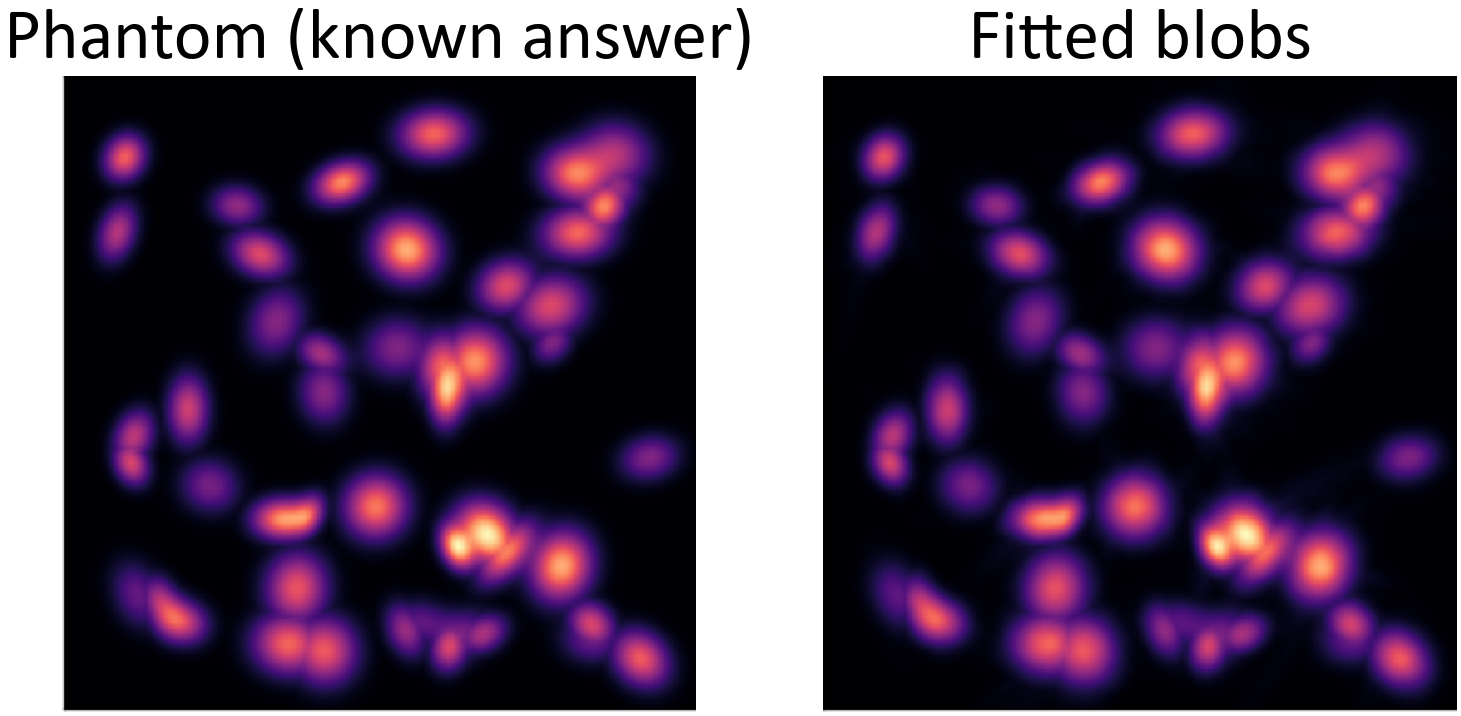
\includegraphics[width=0.72\linewidth]{figs/phantom.png}
  \caption{Step~0. Synthetic phantom (left) and its fit with 2{,}000 Gaussians (right),
  maximum projections; PSNR \SI{47.9}{dB}.}
  \label{fig:phantom}
\end{figure}

\subsection{Step 1 (Akim): start blobs on bright peaks}

\textbf{Change.} Random starting positions were replaced by one blob on each bright local
maximum of the data. \textbf{Why.} A blob that starts far from any structure contributes
nothing and may never reach one. \textbf{Result.} On the phantom (best of 8 fits per setting:
four blob shapes, 50 and 100 blobs), random starts reached \SI{32.0}{dB} and more iterations
added only \SI{1.7}{dB} (\SI{33.7}{dB}); starting on peaks reached \SI{53.1}{dB}, and
\SI{55.1}{dB} with more iterations. Where blobs start mattered far more than how long they were
fitted. Step~7 later explains why.

\subsection{Step 2 (Akim): real data need stretched, rotated blobs}

\textbf{Change.} Moving to real \emph{Tribolium} data (43 experiments, 299 fits), Akim compared
four blob shapes and varied the budget (50--1{,}000 blobs), the voxel sampling, the loss, and an
automatic tuner that estimates background, noise, nucleus size and spacing from the data.
\textbf{Why.} Real nuclei, unlike the phantom, are stretched along $z$, unevenly bright and
tightly packed. \textbf{Result.} The median PSNR rose steeply with shape freedom
(\cref{tab:shapes}). The best fit in the archive reached \SI{25.9}{dB} with 750--1{,}000 blobs on
the whole 37-million-voxel volume; this is the best observed value, not a proven limit. Fixed
round blobs failed largely because their size was fixed at 2 voxels while nuclei need 5--7, so
part of that gap is the constant, not roundness itself.

\begin{table}[tb]
  \centering\small
  \begin{tabular}{@{}lrr@{}}
    \toprule
    Blob shape & Median PSNR (dB), Step~2 & Mean PSNR (dB), Step~5 \\
    \midrule
    Fixed round (size not learned) & 6.8 & --- \\
    Round, learned size & 20.4 & 22.3 \\
    Stretched (axis-aligned) & 23.3 & 25.2 \\
    Stretched and rotated & \textbf{24.0} & \textbf{25.5} \\
    \bottomrule
  \end{tabular}
  \caption{Blob shape on real \emph{Tribolium} data. Step~2: Akim's archive, about 75 fits per
  shape with different budgets and settings, one run each. Step~5: our repeat with 5 seeds and
  3 budgets per shape (15 fits each) on $64\times128\times128$ crops.}
  \label{tab:shapes}
\end{table}

\subsection{Step 3 (Akim): grow blobs where the error is large}

\textbf{Change.} Densification, a standard trick of 3D Gaussian splatting: fitting starts with
25 blobs and splits or clones blobs where the error stays high. Akim tried 12 variants (when to
add blobs, whether new blobs inherit their parent's size and brightness, how many voxels to
sample). \textbf{Why.} The data, rather than a guess, would decide how many blobs are needed.
\textbf{Result.} At similar final numbers of blobs, grown fits were slightly better than fixed
budgets, for example \SI{24.3}{dB} with 34 grown blobs against \SI{23.8}{dB} with 50 fixed
blobs (\cref{fig:densify}). The best grown fits (\SI{24.9}{dB}) used about 165 blobs and
5{,}000 iterations, against \SI{24.5}{dB} for the largest fixed budget (100 blobs, 3{,}000
iterations). The gain is modest, and we kept fixed budgets because they are easier to control
and compare.

\begin{figure}[tb]
  \centering
  \begin{subfigure}[t]{0.44\linewidth}
    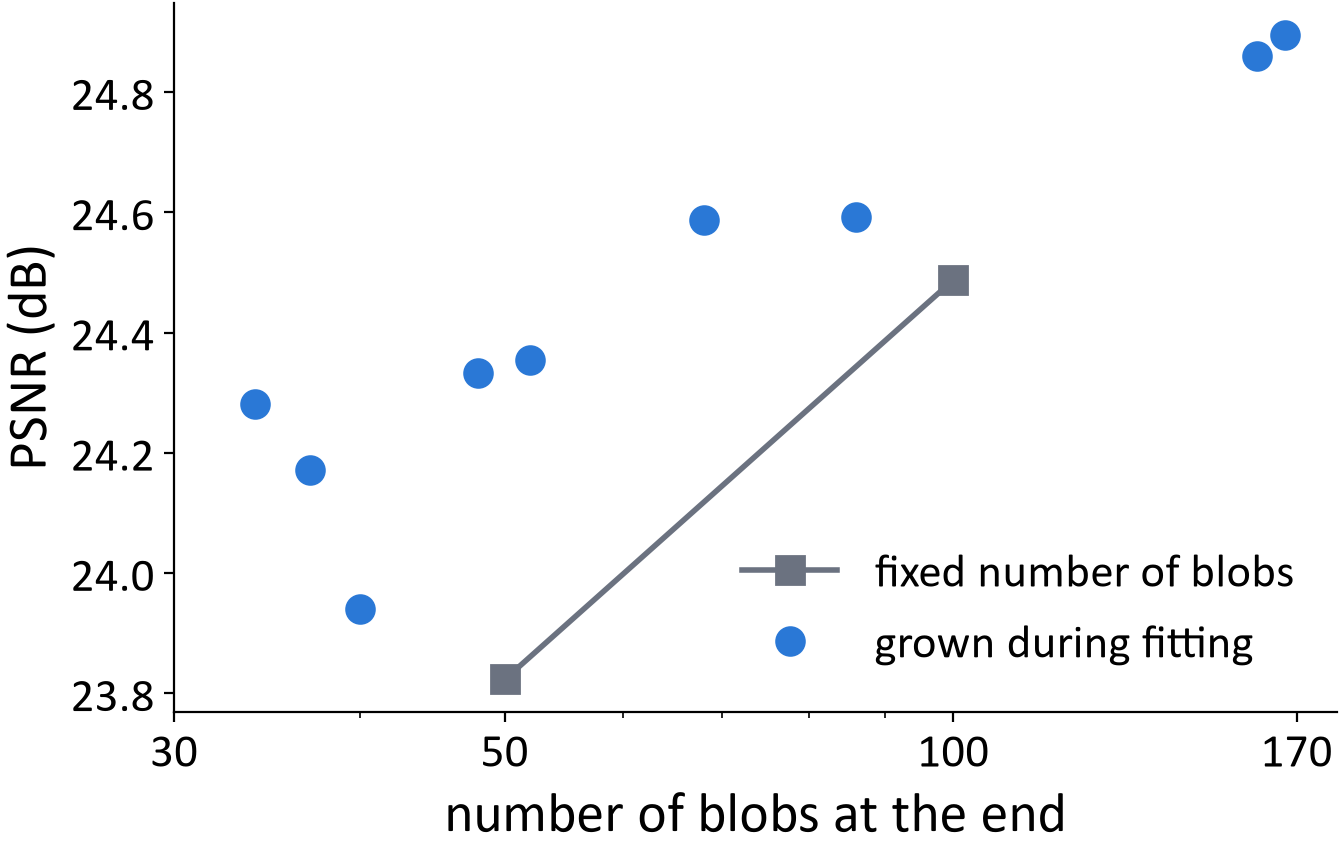
\includegraphics[width=\linewidth]{figs/akim_densify.png}
    \caption{Step~3: densification}
    \label{fig:densify}
  \end{subfigure}
  \hfill
  \begin{subfigure}[t]{0.54\linewidth}
    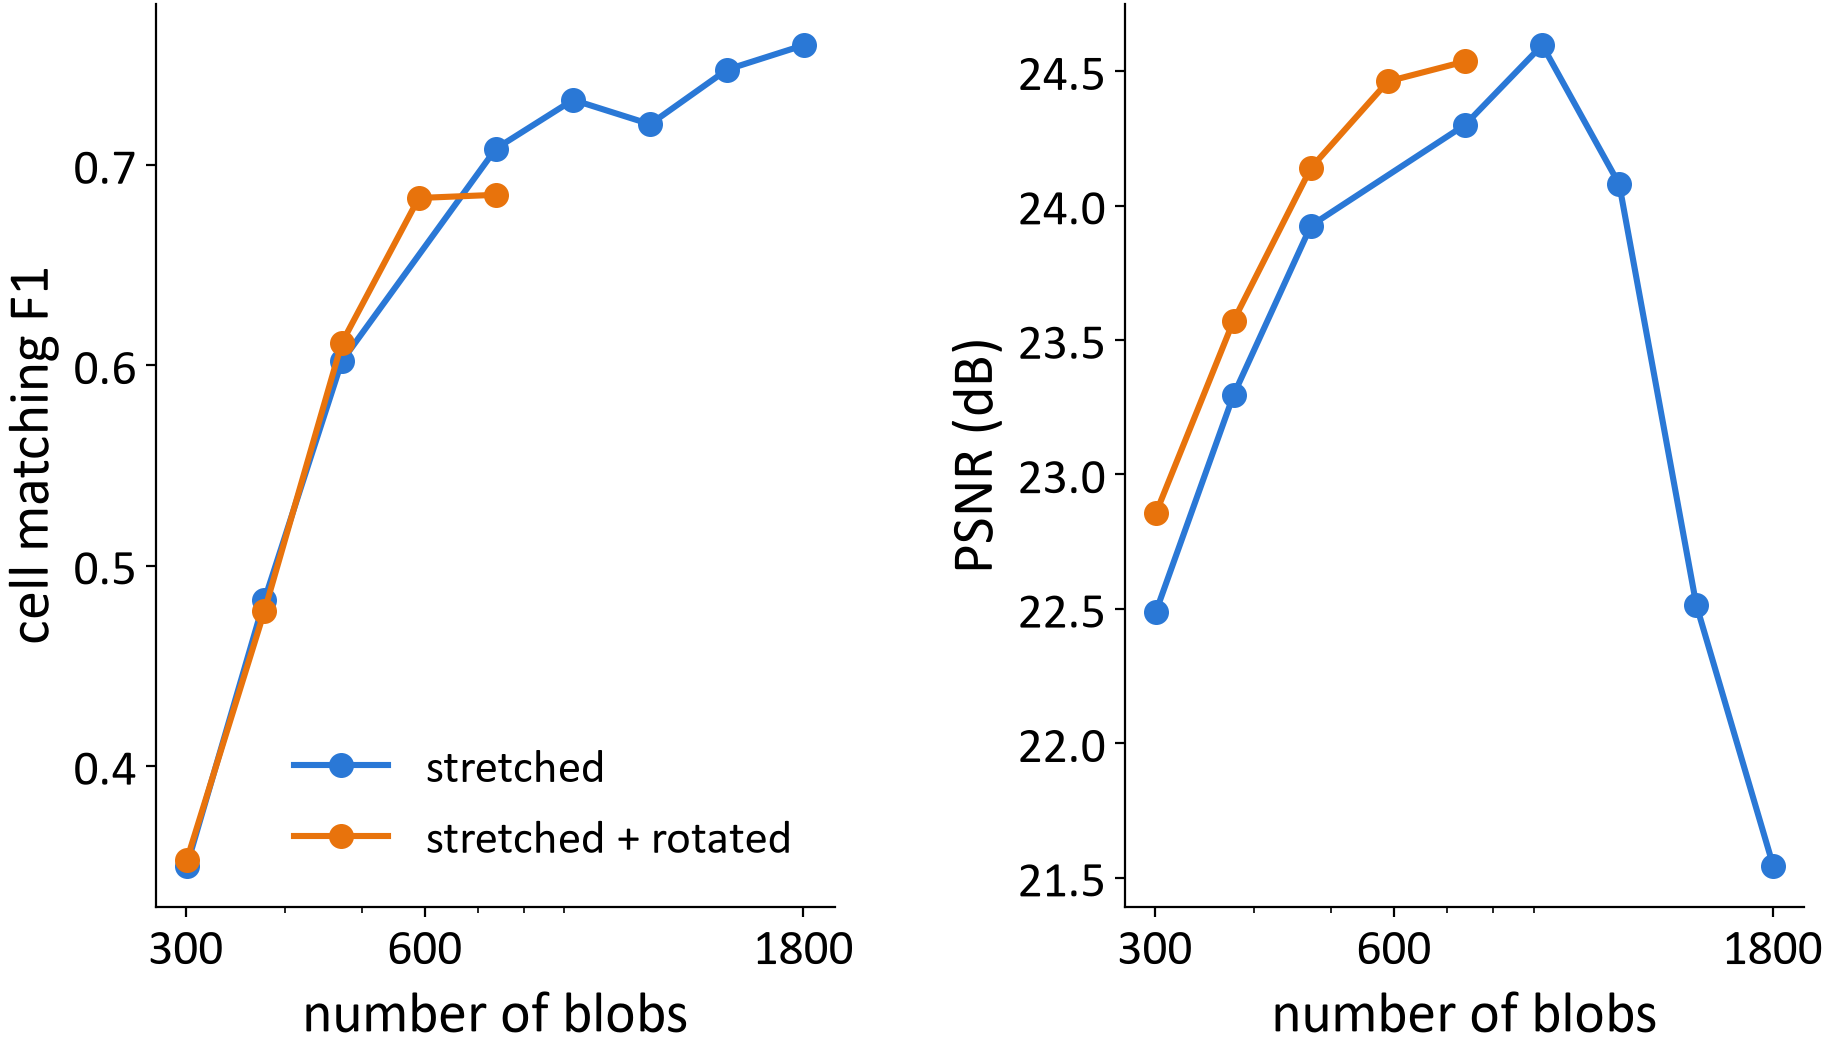
\includegraphics[width=\linewidth]{figs/akim_cellbudget.png}
    \caption{Step~4: budget from the cell count}
    \label{fig:cellbudget}
  \end{subfigure}
  \caption{Akim's experiments on \emph{Tribolium}. (a)~PSNR against the final number of blobs,
  same crop, stretched and rotated blobs: fits grown during fitting (dots) and fixed budgets
  (squares). (b)~Whole volume, budgets set from 230 detected cells: agreement between peaks of
  the reconstruction and the detected cells (left, F1) and PSNR (right). All runs stopped after
  3{,}000 iterations, which under-trains the largest budgets.}
  \label{fig:akim}
\end{figure}

\subsection{Step 4 (Akim): set the budget from the cell count}

\textbf{Change.} Instead of guessing $K$, a detector first counted about 230 cells in the whole
volume; the budget was then 1.15 blobs per cell plus 12\% for background (301 blobs), and
multiples of it. \textbf{Why.} If every cell gets a blob, the blobs should match the cells.
\textbf{Result.} Agreement between peaks of the reconstruction and the detected cells rose
steadily with the budget, from F1 0.35 at 301 blobs to 0.76 at 1{,}804 (\cref{fig:cellbudget}).
PSNR, however, peaked near 900 blobs and then fell, because every run stopped after 3{,}000
iterations. This was the first sign that image quality and finding cells do not always agree.
The F1 gain comes with a sixfold larger budget: it shows that more blobs match more cells, not
that deriving the budget from the cell count is better than another way of choosing it, which
was not compared. The reference cells here come from a detector, not from people.

\subsection{Step 5 (ours): repeats confirm that stretching is real}

\textbf{Change.} We re-ran round, stretched, and stretched-and-rotated blobs with 5 random seeds
and 3 budgets each. \textbf{Why.} Akim's archive had one run per setting, and a single run can be
luck. \textbf{Result.} Stretching held up: \SI{22.3}{dB} (round), \SI{25.2}{dB} (stretched),
\SI{25.5}{dB} (stretched and rotated), averaged over budgets of 50, 100 and 250 blobs
(\cref{tab:shapes}). The ordering held at every budget, and the standard deviation over seeds
was 0.02--\SI{0.13}{dB} within each shape and budget, far below the \SI{3}{dB} effect.
Most of the gain comes from stretching; rotation adds about \SI{0.3}{dB}. Nucleus F1 against
detector-derived references rose from 0.745 to 0.805 (paired test over 5 seeds, $p=0.006$). The
learned blobs were also about as stretched as the real nuclei: depth-to-width ratio 0.79 against
0.73 measured on the nuclei.

\subsection{Step 6 (ours): start one blob on every nucleus}

\textbf{Change.} Peak starts (Step~1) were replaced by a start that first places one blob on
every detected nucleus and then fills the remaining budget. \textbf{Why.} We measured that blobs
travelled less than one voxel on average during fitting, while nuclei are about 20 voxels apart,
so a blob that starts between nuclei stays there. With brightest-peak starts, bright background
crowded out faint nuclei. \textbf{Result.} Over four \emph{Tribolium} regions (110 nuclei) the
share of nuclei with a blob at the start rose from 73\% to 100\%, and the share found after
fitting from 52\% to 71\%. These references come from a related detector, so this result is
partly circular; on human-labelled \emph{Drosophila} the specific window rule did not transfer,
whereas setting all windows in micrometres did.

\subsection{Step 7 (ours): larger position steps let blobs travel}

\textbf{Change.} We raised the learning rate of blob positions by up to $62\times$.
\textbf{Why.} The default had been copied from photographic 3D splatting code, where coordinates
are small, and was never rescaled to voxel coordinates. \textbf{Result.} Blobs started to move
between nuclei (\cref{tab:lr}). With bad starts this closed the gap completely (F1 0.64 $\to$
0.78), but with good starts it hurt (0.84 $\to$ 0.78). The position optimiser had been
under-scaled rather than trapped in local minima, which is why starting positions mattered so
much in Steps~1 and~6. Good starts with the default step remained best.

\begin{table}[tb]
  \centering\small
  \begin{tabular}{@{}lrrrr@{}}
    \toprule
    Position          & Mean travel & Moved to another & F1 gap (good    & F1, good \\
    learning rate     & (voxels)    & nucleus          & $-$ random starts) & starts \\
    \midrule
    0.0016 (default, $1\times$) & 0.96 & 1.0\% & $+0.207$ & 0.842 \\
    0.005 ($3\times$) & 2.47 & 5.5\% & $+0.169$ & --- \\
    0.016 ($10\times$) & 5.81 & 14.5\% & $+0.155$ & --- \\
    0.05 ($31\times$) & 10.76 & 28.0\% & $+0.048$ & --- \\
    0.1 ($62\times$) & 14.79 & 32.0\% & $+0.001$ & 0.776 \\
    \bottomrule
  \end{tabular}
  \caption{Step~7: position learning rate (\emph{Tribolium}, 100 blobs, 3{,}000 iterations, 2
  seeds). A blob \emph{moved to another nucleus} if its nearest nucleus changed during fitting.
  F1 against detector-derived references.}
  \label{tab:lr}
\end{table}

\subsection{Step 8 (ours): cap the size of nucleus blobs}

\textbf{Change.} An upper limit of 10 voxels on the scale of the blobs that started on nuclei
(\SI{6.9}{\micro\meter} in $xy$ but \SI{30}{\micro\meter} in $z$, so in effect a cap in $xy$). \textbf{Why.} The nuclei still
lost were the faint ones. At the end of fitting, the blob nearest to each lost nucleus was not
dimmer than for kept nuclei (amplitude $p=0.63$) but wider (scale 11.7 against 9.1 voxels,
$p=0.001$), and a wide blob leaves only a flat peak for a detector to find. A cap on width
should therefore help. This is an association at the end of fitting, not a tracked trajectory
of individual blobs, and it was scored before the matcher fix (\cref{app:bugs}) and could not
be rescored. \textbf{Result.} Faint nuclei found
rose from 13 to 19 of 31 and overall recall from 0.730 to 0.800, while global PSNR changed by
\SI{-0.012}{dB} (\cref{tab:cap,fig:cap}). The result rests on one seed and four regions, one
region got worse, and on human-labelled \emph{Drosophila} the cap changed nothing because it
bound only 2\% of blobs there. It is promising, not settled.

\begin{table}[tb]
  \centering\small
  \begin{tabular}{@{}lccccc@{}}
    \toprule
     & Region 1 & Region 2 & Region 3 & Region 4 & Pooled \\
    \midrule
    No cap & 4/9 & 5/13 & 3/4 & 1/5 & 13/31 \\
    Cap 10 voxels & 5/9 & 9/13 & 2/4 & 3/5 & \textbf{19/31} \\
    \bottomrule
  \end{tabular}
  \caption{Step~8: faint nuclei still detected after fitting, four \emph{Tribolium} regions,
  seed 0, default position learning rate. Overall recall (mean over regions) 0.730 $\to$ 0.800;
  global PSNR 24.758 $\to$ \SI{24.746}{dB}.}
  \label{tab:cap}
\end{table}

\begin{figure}[tb]
  \centering
  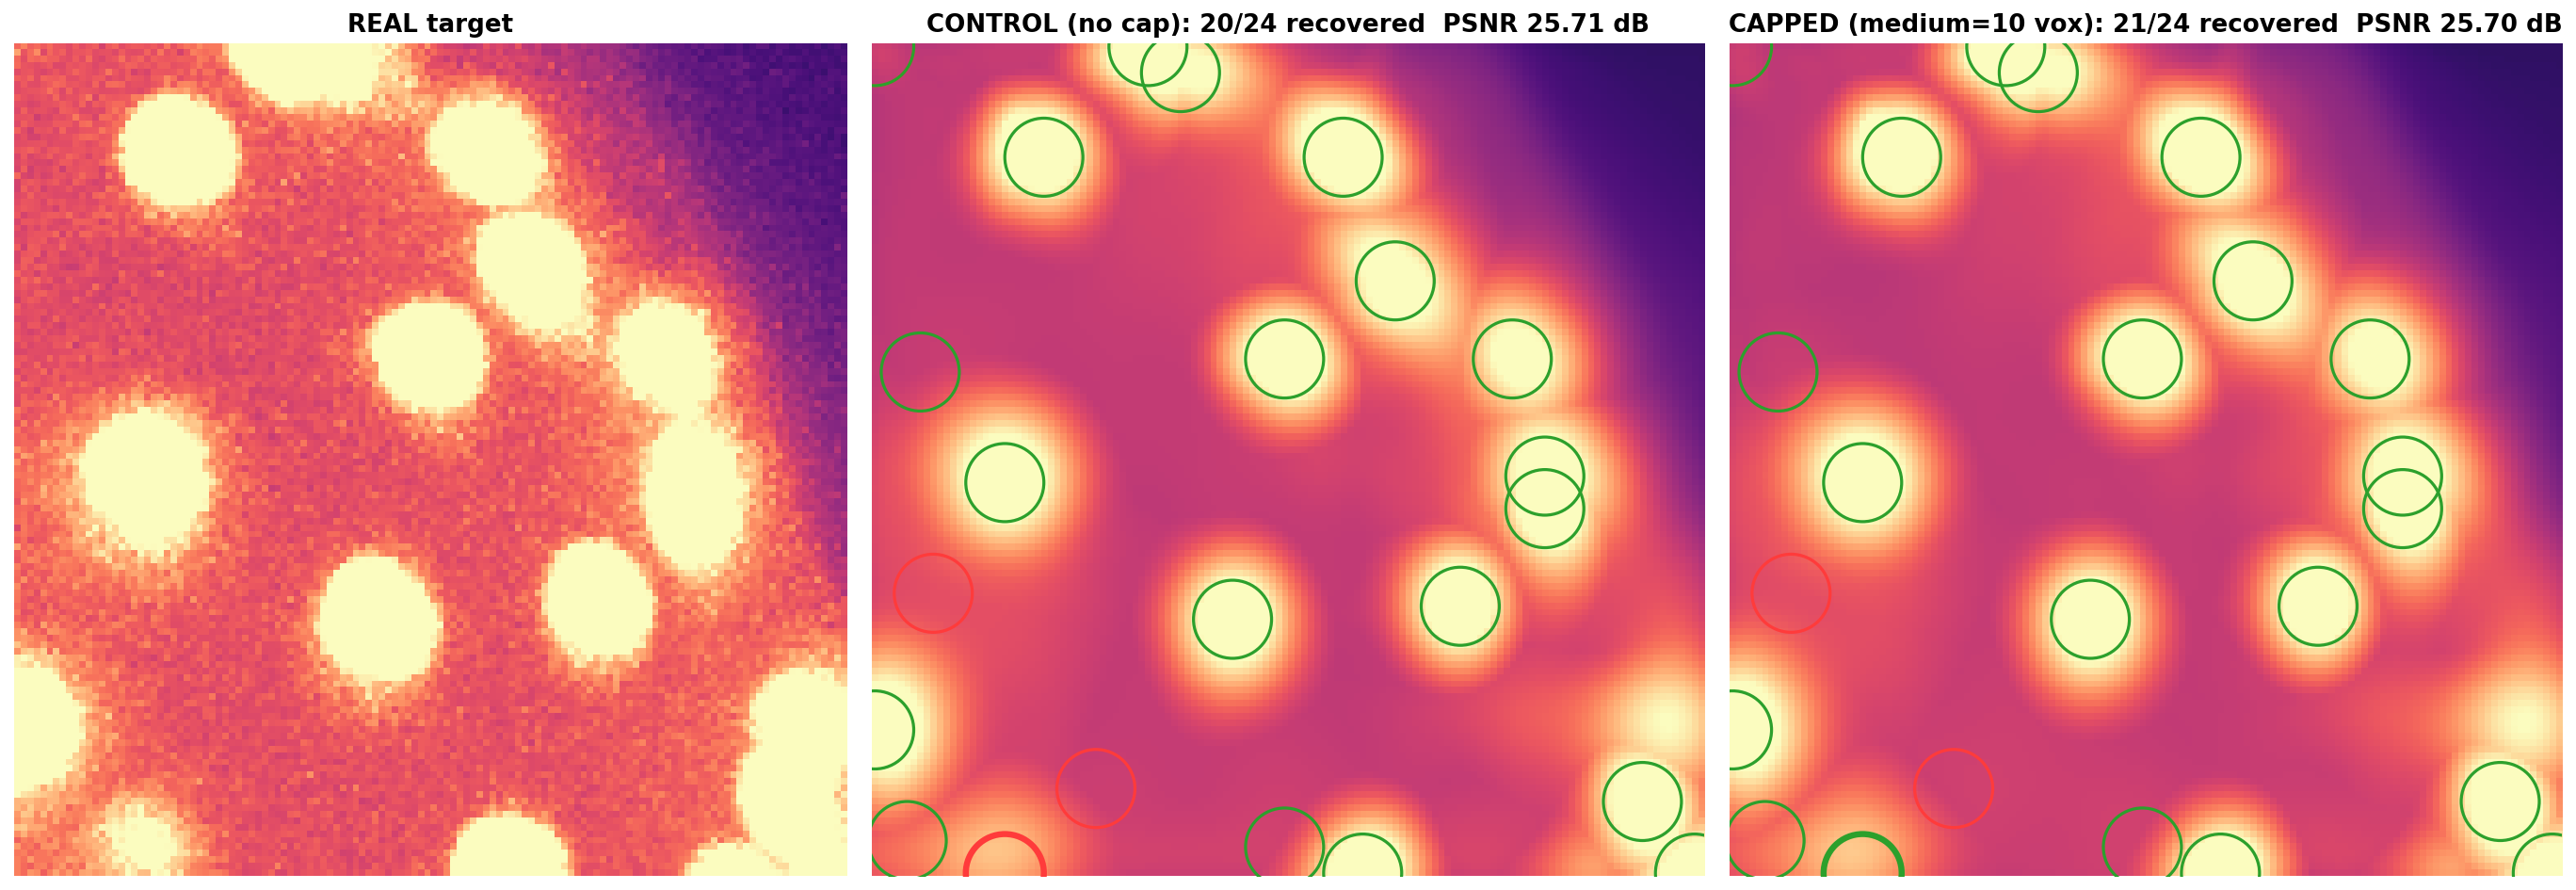
\includegraphics[width=\linewidth]{figs/tribolium_control_vs_capped.png}
  \caption{Step~8 on one \emph{Tribolium} crop with 24 detector-found nuclei. Left: data
  (maximum projection). Middle: fit without cap, 20 of 24 nuclei recovered. Right: capped fit,
  21 of 24. PSNR 25.71 against \SI{25.70}{dB}.}
  \label{fig:cap}
\end{figure}

\subsection{Why faint nuclei are lost}\label{sec:mechanism}

Two measurements explain much of what the steps above fought against. First, most of the blob
budget models background: in two regions with 250 blobs each, 62 of 63 nuclei were covered by
exactly one blob, but only 31--33 blobs sat on a nucleus, carrying 10--17\% of the total
amplitude; the remaining 87\% of blobs model a near-constant background. Under squared error a
missed faint nucleus costs far less than a small error spread over the background, so the
objective rationally spends capacity there. A learnable background term did not help, because
with 250 broad blobs the split between the term and the blobs is not identifiable. Second, the
blobs associated with lost faint nuclei at the end of fitting were wider than those of kept
nuclei, and capping their width improved retention (Step~8). This supports broadening as a
contributor to losing faint nuclei under this fitting regime. We do not claim a proven causal
chain: the comparison uses the blob nearest to each nucleus at the end of fitting, not blobs
tracked through fitting.

\subsection{From the simple setup to the final recipe}

\Cref{tab:recipe} lists all eight changes. They are separate comparisons under the settings
stated in each step, not a chain in which each row builds on the one before. They used
different data, budgets and numbers of repeats, so they cannot be added up into one overall
improvement, and row~4 compares budgets, not ways of choosing a budget. The final recipe is: stretched and rotated
blobs, one starting blob per detected nucleus, the default position learning rate with these
good starts, and a size cap for nucleus blobs. A combination of a larger learning rate with the
cap was never run and is not part of the recipe.

\begin{table}[tb]
  \centering\small
  \begin{tabular}{@{}llllrr@{}}
    \toprule
    Step & Change & By & Measured as & Before & After \\
    \midrule
    1 & Start on bright peaks & Akim & PSNR, phantom (best of 8) & 32.0\,dB & 53.1\,dB \\
    2 & Stretched + rotated blobs & Akim & PSNR, real data, median & 20.4\,dB & 24.0\,dB \\
    3 & Grow blobs during fitting & Akim & PSNR, 34 grown vs 50 fixed & 23.8\,dB & 24.3\,dB \\
    4 & Budget in cell-count units & Akim & cell-matching F1, 301 $\to$ 1{,}804 blobs & 0.35 & 0.76 \\
    5 & Repeat of the shape test & ours & PSNR, 15 fits per shape & 22.3\,dB & 25.5\,dB \\
    6 & One start per nucleus & ours & nuclei found, of 110 & 52\% & 71\% \\
    7 & Larger position steps & ours & F1, random starts & 0.64 & 0.78 \\
    8 & Size cap & ours & faint nuclei found, of 31 & 13 & 19 \\
    \bottomrule
  \end{tabular}
  \caption{The eight changes from the naive setup (round blobs, random starts, default steps,
  no cap): separate comparisons under the settings stated in each step. The rows are not
  cumulative. Row~4 shows F1 as the budget grows sixfold; it does not compare the cell-count rule
  with another way of choosing the budget.}
  \label{tab:recipe}
\end{table}

% =====================================================================
\section{Validation: does the fit behave as expected?}\label{sec:validation}
% =====================================================================

\paragraph{Shape.} The learned blobs are about as stretched as the real nuclei (depth-to-width
ratio 0.79 against 0.73), as expected if they describe nuclei rather than arbitrary texture.

\paragraph{Human labels.} The \emph{Tribolium} references above come from a detector, so a fit
can look good by agreeing with it. We therefore tested on 29 human-labelled \emph{Drosophila}
nuclei in one $64\times128\times128$ crop. All fits started from the same 457 detector
candidates of the raw volume, so only the fitting differed, and methods were compared at the
same number of detections (\cref{tab:human,fig:human}). Fitting ranked true nuclei above image
brightness in every seed (14 against 10 of 29 in the top 100). But a scale-normalised LoG filter
applied to the same raw candidates did better in the top 100 (16--18), in seconds; in the top
200 the best fit and the filter were level (22.7 against 22, within one nucleus). The raw
detector using all 457 candidates found 26 of 29, more than any fit. The fit's advantage over brightness is
explained by blob-shaped scoring, not by anything specific to the Gaussian representation. A
large position learning rate hurt good starts here too, as \cref{tab:lr} predicts, and the
best-PSNR fit found fewer nuclei in the top 100 than the default fit: image quality and object
fidelity come apart. With 29 labels one nucleus is 3.4 recall points, so we call a difference
real only if it is about three nuclei or more and has the same sign in every seed.

\begin{table}[tb]
  \centering\small
  \begin{tabular}{@{}lccl@{}}
    \toprule
    Method & Top 100 & Top 200 & Notes \\
    \midrule
    Raw volume, ranked by brightness & 10 & 18 & 26/29 using all 457 candidates \\
    Downsampled to similar storage & 10 & 11 & \SI{17.9}{dB} vs.\ \SI{21.5}{dB} for the fit \\
    Gaussian fit, default & 14.0 & 21.0 & best single fit reaches 23 \\
    \quad + size cap (17 voxels) & 14.0 & 21.0 & cap binds 2\% of blobs \\
    \quad + uniform sampling & 11.7 & 22.7 & best PSNR of all fits ($+0.4$\,dB) \\
    \quad + large position learning rate & 11.0 & 18.3 & \\
    \midrule
    Raw candidates, LoG multi-scale (1.5--\SI{3}{\micro\meter}) & \textbf{16} & \textbf{22} & seconds, deterministic \\
    Raw candidates, LoG \SI{2}{\micro\meter} & \textbf{18} & \textbf{22} & scale chosen after seeing results \\
    \bottomrule
  \end{tabular}
  \caption{Human-labelled \emph{Drosophila} nuclei (of 29) among the top-$N$ detections. Fit rows
  are means of 3 seeds. Paired per-seed differences, fit minus raw brightness: $+3, +5, +4$ (top
  100) and $+2, +4, +3$ (top 200).}
  \label{tab:human}
\end{table}

\begin{figure}[tb]
  \centering
  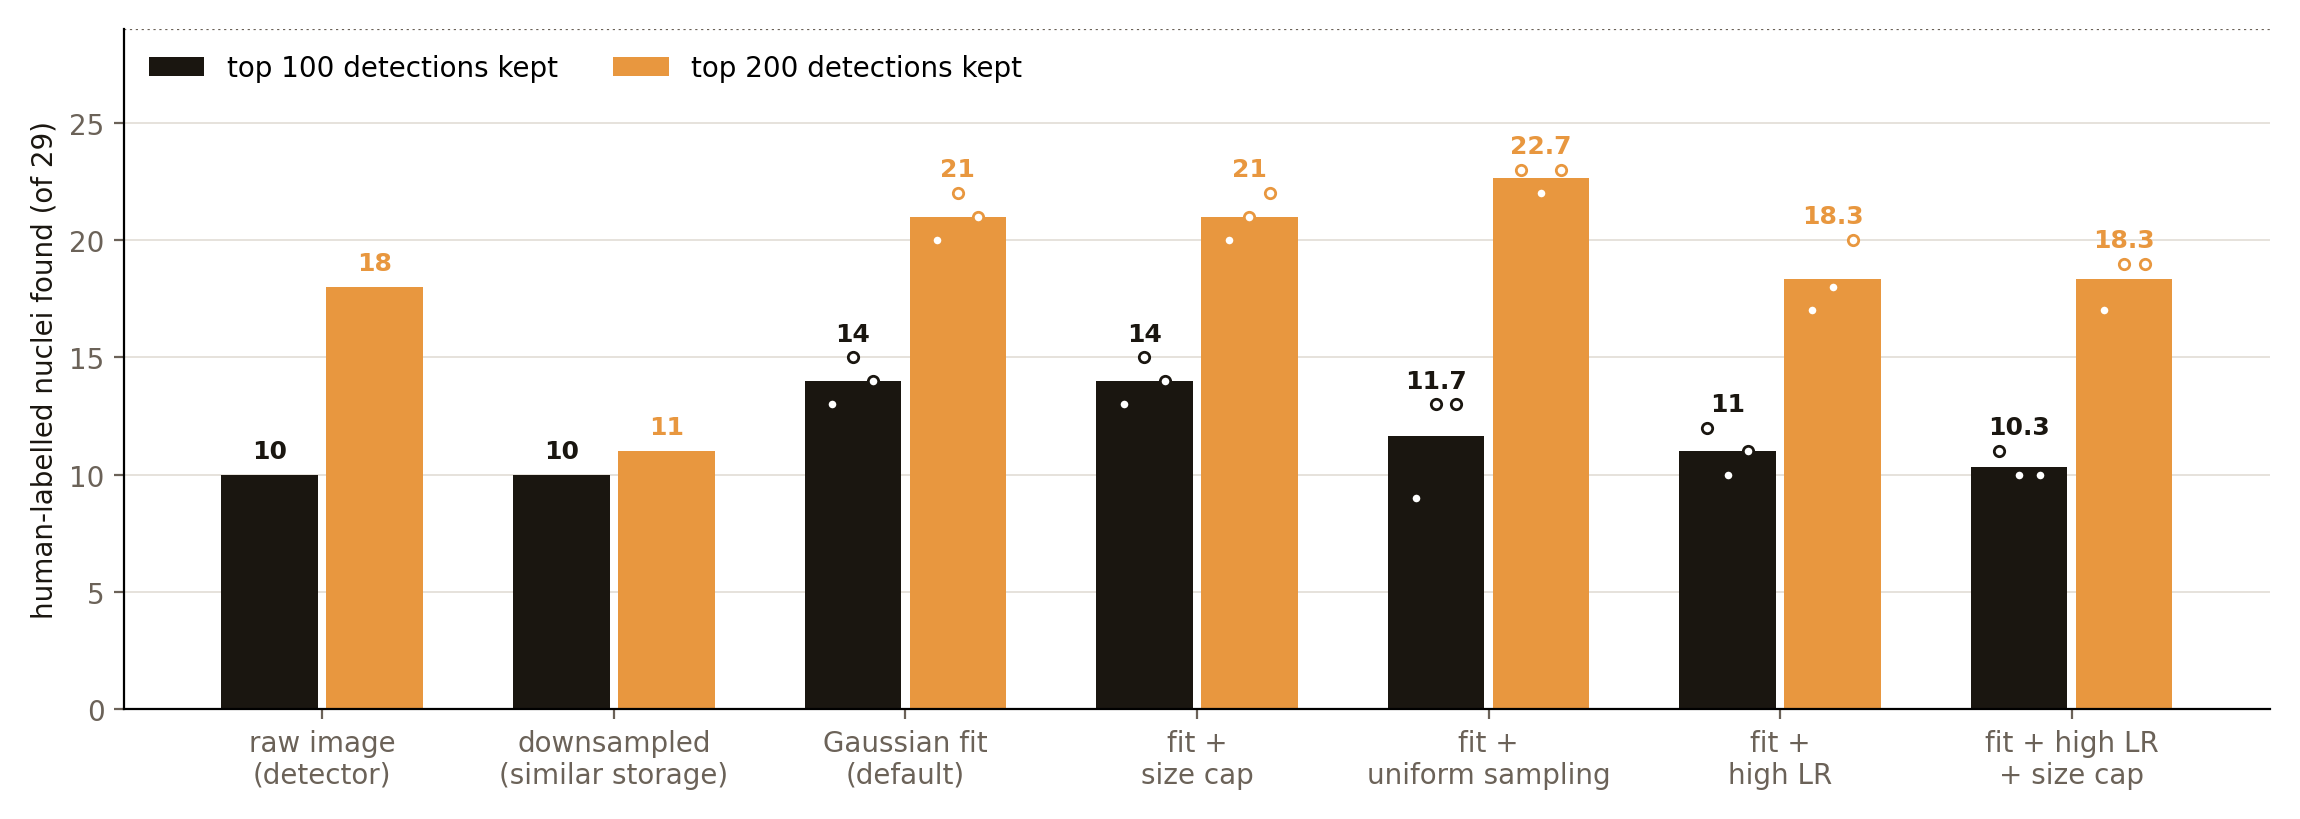
\includegraphics[width=\linewidth]{figs/drosophila_human_label_check.png}
  \caption{Human-labelled nuclei found in the top 100 and top 200 detections per method (bars:
  mean; dots: seeds). The LoG baseline of \cref{tab:human} is not drawn: it exceeds every fit
  in the top 100 (16--18), and in the top 200 (22) it is level with the uniform-sampling fit
  (22.7).}
  \label{fig:human}
\end{figure}

\paragraph{Repeatability.} Repeated fits differ little: in Step~5 the spread between seeds was
small against the \SI{3}{dB} shape effect, and three independent Luxar fits of the same frame
(\cref{sec:sota}) differed by at most \RepLoG--\RepCP{} points of nuclei kept.

\paragraph{Naive baselines for other uses.} We also tested whether the fitted representation
helps beyond storage. Every use lost to a simple baseline (\cref{tab:neg}), which motivated
the comparison with the state of the art in the next section.

\begin{table}[tb]
  \centering\small
  \begin{tabularx}{\linewidth}{@{}l>{\raggedright\arraybackslash}X@{}}
    \toprule
    Use & Outcome \\
    \midrule
    Compression & Blobs lead at very small budgets (1{,}000 numbers: 23.4 vs.\ \SI{21.6}{dB}),
      but plain downsampling catches up by about 10{,}000 numbers (23.1 vs.\ \SI{23.3}{dB}).
      Going from 100 to 2{,}000 blobs bought only \SI{0.36}{dB}. \\
    Detection & The raw detector with all candidates finds more; LoG ranks better (\cref{tab:human}). \\
    Tracking by persistence & A plain detect-then-link tracker already keeps 76--83\% of the 189
      annotated tracks over 20 frames; linking real detections is 96.2\% correct. \\
    Axial super-resolution & Linear and cubic interpolation were as good (not run head-to-head
      on identical held-out slices). \\
    Time series & Sharing blob identities over time used $3.4\times$ \emph{more} parameters
      (13{,}200 vs.\ 3{,}900), not fewer. \\
    Cell divisions & Untestable: none of the annotated tracks divide. \\
    \bottomrule
  \end{tabularx}
  \caption{Other uses of the representation that were tested and lost to a simple baseline.}
  \label{tab:neg}
\end{table}

% =====================================================================
\section{Comparison with the state of the art at matched file size}\label{sec:sota}
% =====================================================================

Our own fits improved on the naive setup, but they are slow (minutes per small crop on a CPU)
and were never designed for whole recordings. If Gaussian blobs are to win anywhere, the
strongest existing tool must win. We therefore compared Luxar~\cite{royer2026luxar} with
standard codecs at identical file size on the \emph{C.~elegans} frames, scored by four detectors
against human labels.

\subsection{Setup}

\paragraph{Compressors.} Luxar with its default settings, 1{,}000 iterations and anisotropic
voxel size, at budgets $K$ from 500 to $6.4\times10^4$ splats; its size is the
\texttt{.gsplats.zarr} store on disk, metadata included. Renders are mapped to raw intensities
by a least-squares gain and offset (two numbers, not counted, which slightly favours Luxar). We
also ran Luxar's own calibration, a blind-spot held-out PSNR~\cite{batson2019noise2self}, to
obtain its recommended budget $K^\ast$. JPEG2000 (OpenJPEG) codes each $xy$ slice with a 2D
wavelet, slices stored as components of one codestream, and is bisected to \emph{exactly} the
bytes of every Luxar fit. JPEG-XL codes each slice and is bisected to 50--800\,KiB.

\paragraph{Detectors.} (a)~LoG: local maxima ranked by scale-normalised LoG response
at scales $\sigma = 0.2D$, $0.27D$, $0.33D$ and $0.4D$, top $N$ kept, $N$ = number of labels. (b)~Watershed:
background-subtracted, Otsu-thresholded foreground split by a distance-transform watershed in
physical units, parameters fixed on raw volumes. (c)~Cellpose~3 \emph{nuclei} model, 2D per
slice stitched across $z$, and (d)~the same model in its 3D mode. On the raw volumes they find
\RecallLoG, \RecallWS, \RecallCP{} and \RecallCPthree{} of the labelled nuclei. Detections match
labels one-to-one within $0.6D$; \cref{tab:radius} varies the radius.

\paragraph{Statistics.} Each frame counts once: per-frame mean difference between Luxar and
JPEG2000 at identical bytes, Wilcoxon signed-rank tests over the 12 frames, Holm-corrected over
the eight detector--regime comparisons, and 95\% cluster-bootstrap intervals over frames.
Pass/fail rules were written down and committed before each new measurement
(\cref{app:rules}); the two that failed are reported as failed.

\paragraph{A baseline pitfall.} Passing a $(z,y,x)$ array to a common JPEG2000 binding encodes a
$z$--$y$ image with one component per $x$ column, so the wavelet never runs along $x$. That
configuration, which we used at first, cost about \SI{10}{dB} at \SI{220}{\times} and made
splats appear far better than JPEG2000 beyond \SI{200}{\times}. Fixing it reversed our first
conclusion. A regression test now checks the codestream header.

\subsection{Results}

\begin{figure}[tb]
  \centering
  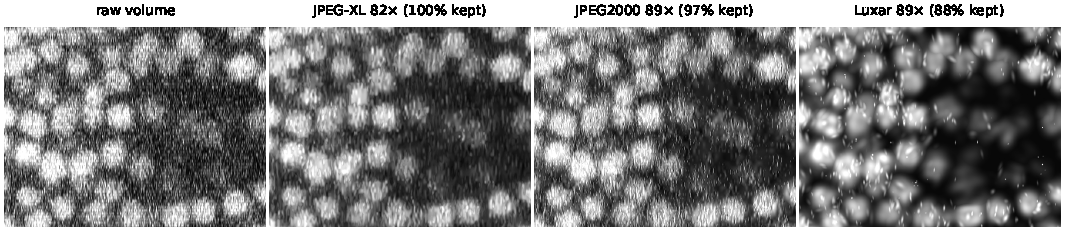
\includegraphics[width=\linewidth]{figs/fig_qualitative.pdf}
  \caption{The same region of embryo~1, t194 (3-slice maximum projection) from the raw
  volume, JPEG-XL, and JPEG2000 and Luxar at identical bytes; titles give whole-frame nuclei
  kept by 2D Cellpose. Both codecs keep the texture of nuclei; Luxar renders smooth blobs on a
  black background with thin streaks from elongated splats.}
  \label{fig:qual}
\end{figure}

\paragraph{PSNR says JPEG2000; the detectors say it depends.} JPEG2000 had higher PSNR on every
frame in both regimes and in all \PSNRjtkWins{} pairs, by \DPSNR{} (\cref{tab:main}). Below
\SI{300}{\times}, 3D Cellpose favoured the splats (Luxar $-$ JPEG2000 = \FrModCPthree{} points
of nuclei kept, \FrModCPthreePos{} of \FrN{} frames, $p_\mathrm{Holm}=\FrModCPthreeP$), whereas
the watershed and 2D Cellpose favoured JPEG2000 (\FrModWS{} and \FrModCP{} points, every frame,
$p_\mathrm{Holm}=\FrModWSP$ and \FrModCPP). The LoG detector showed no consistent difference
(\FrModLoG{} points, \FrModLoGPos{} of \FrN{} frames, $p_\mathrm{Holm}=\FrModLoGP$); it favoured
splats on embryo~2 (\FrModLoGETwo) but not on embryo~1 (\FrModLoGEOne). Beyond
\SI{300}{\times} (up to \JtkMaxRatio) every detector favoured JPEG2000 on \FrFarNeg{} of \FrN{}
frames, by \FrFarLoG{} (LoG) to \FrFarCP{} (2D Cellpose) points, while JPEG2000 still kept
\FarJtkLoG{} (LoG) and \FarJtkWS{} (watershed) of nuclei. Every individual pair is shown in
\cref{fig:matched}. JPEG-XL was nearly lossless up to its maximum distance (\JXLmax; worst case
\JXLworst).

\begin{table}[tb]
  \centering
  \setlength{\tabcolsep}{5pt}
  \begin{tabular}{lrcrc}
\toprule
 & \multicolumn{2}{c}{below \SI{300}{\times}} & \multicolumn{2}{c}{\SI{300}{\times} and beyond} \\
\cmidrule(lr){2-3}\cmidrule(lr){4-5}
Luxar $-$ JPEG2000 & mean [95\% CI] & L\,:\,J & mean [95\% CI] & L\,:\,J \\
\midrule
PSNR (dB) & $-$2.4 [$-$2.7, $-$2.1] & 0\,:\,12 & $-$1.4 [$-$1.6, $-$1.3] & 0\,:\,12 \\
\midrule
LoG & +1.3 [+0.0, +2.7] & 8\,:\,4 & \textbf{$-$16.6} [$-$23.0, $-$10.2] & 1\,:\,11 \\
Watershed & \textbf{$-$4.0} [$-$5.3, $-$2.7] & 0\,:\,12 & \textbf{$-$19.3} [$-$23.8, $-$15.0] & 0\,:\,12 \\
Cellpose (2D) & \textbf{$-$9.4} [$-$11.4, $-$7.3] & 0\,:\,12 & \textbf{$-$23.2} [$-$28.0, $-$18.3] & 0\,:\,12 \\
Cellpose (3D) & \textbf{+3.5} [+1.8, +5.5] & 10\,:\,2 & \textbf{$-$18.2} [$-$23.8, $-$12.8] & 0\,:\,12 \\
\bottomrule
\end{tabular}

  \caption{Luxar minus JPEG2000 at identical bytes, frame level: mean over \FrN{} frames of the
  per-frame mean difference (nuclei kept in percentage points; PSNR in dB), 95\%
  cluster-bootstrap interval over frames, and frames favouring Luxar\,:\,JPEG2000 (L\,:\,J).
  Bold: Holm-corrected Wilcoxon $p<0.05$.}
  \label{tab:main}
\end{table}

\begin{figure}[tb]
  \centering
  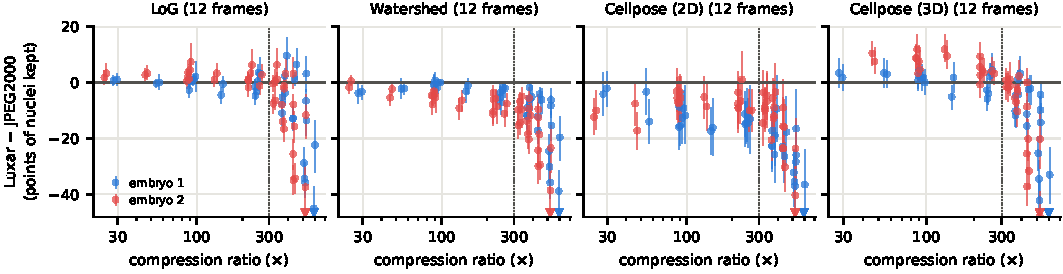
\includegraphics[width=\linewidth]{figs/fig_matched.pdf}
  \caption{Every Luxar fit against JPEG2000 at identical bytes: difference in nuclei kept
  (points; bars: 95\% bootstrap intervals over nuclei) for the four detectors. Above zero,
  splats keep more nuclei; triangles: below $-48$ points. Dotted line: \SI{300}{\times}.}
  \label{fig:matched}
\end{figure}

\paragraph{Why the detector matters.} Smooth splats can act as a denoiser for detectors that pool
over a volume: under LoG and 3D Cellpose, nuclei kept often exceeded 100\% (Luxar at
\SIrange{45}{94}{\times}: \LuxMidLoG{} and \LuxMidCPthree). Per-slice and threshold-based
segmenters instead see smooth blobs on a black background with streaks (\cref{fig:qual}). The
same Cellpose network shows this cleanly. At \SIrange{45}{94}{\times}, JPEG-XL minus splats was
\GapCP{} points of nuclei kept in 2D mode but \GapCPthree{} in 3D mode, where the 5-point
penalty we had tested for in advance appeared on \RuleGapBigCPthree{} frames. The same weights
behave differently, so the penalty is not a fixed property of the learned model; this supports
an explanation involving processing geometry (slices versus the whole volume). The 3D mode also
combines and post-processes predictions differently, so switching modes establishes the
difference in behaviour but does not isolate its exact cause. The watershed sits in between
(\GapWS{} points; under the pre-set 5 points on \RuleGapSmallWS{} frames).

\paragraph{The budget cliff.} Splats lose nuclei abruptly once they become scarce
(\cref{fig:cliff}): under LoG, nuclei kept fell below 90\% at \CrossRange{} splats per labelled
nucleus on all \NFrames{} frames, as pre-registered ($\le3.5$). Over budgets $K\ge1000$, Luxar's
PSNR varied by at most \LuxPSNRspan{} per frame. Our pre-registered test that PSNR misses the
cliff within $K$ = 1{,}000--16{,}000 held on only \RulePsnrOK{} added frames: on smaller frames
the cliff lies below that range. Survival, the share of the raw volume's 100 strongest LoG
detections still found, needs no labels and tracks nuclei kept across fits (Spearman
$\rho=\SurvRho$, $n=\SurvN$), so it can flag the cliff.

\begin{figure}[tb]
  \centering
  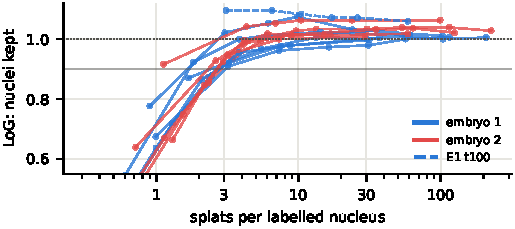
\includegraphics[width=0.62\linewidth]{figs/fig_cliff.pdf}
  \caption{The budget cliff: LoG nuclei kept against splats per labelled nucleus, every Luxar
  fit on all frames (dashed: embryo~1, t100).}
  \label{fig:cliff}
\end{figure}

\paragraph{Luxar at its own budget.} Luxar's calibration recommended $K^\ast=\Kstar$ on all
\KstarCalFrames{} calibrated frames of both embryos, the top of our grid, with held-out PSNR
still rising. There, at \KstarRatio, it kept \KstarLoG{} (LoG), \KstarWS{} (watershed),
\KstarCP{} (2D Cellpose) and \KstarCPthree{} (3D Cellpose) of nuclei; JPEG2000 at the same
bytes kept \KstarJtk, in seconds rather than \FitA{} of fitting per volume on an A100 GPU
(\FitH{} on an H100).

\paragraph{Robustness.} Three independent Luxar fits of embryo~1 t194 at each of three budgets
differed by at most \RepLoG{} (LoG), \RepWS{} (watershed) and \RepCP{} (2D Cellpose) points.
The conclusions do not depend on the match radius (\cref{tab:radius}). On embryo~1 t100, with
larger early nuclei, LoG favoured splats more strongly (\EarlyAdvPts{} points at
\EarlyAdvRatio).

\begin{table}[tb]
  \centering\small
  \begin{tabular}{lcccccc}
\toprule
 & \multicolumn{3}{c}{LoG} & \multicolumn{3}{c}{Cellpose (2D)} \\
\cmidrule(lr){2-4}\cmidrule(lr){5-7}
Radius & raw & JXL & Luxar & raw & JXL & Luxar \\
\midrule
0.4$D$ & 1009 & 1.00 & 1.02 & 658 & 1.01 & 0.84 \\
0.6$D$ & 1032 & 1.00 & 1.01 & 788 & 0.97 & 0.88 \\
0.8$D$ & 1034 & 1.00 & 1.01 & 796 & 0.99 & 0.90 \\
\bottomrule
\end{tabular}

  \caption{Match-radius sensitivity (four first frames): nuclei found in the raw volumes and
  nuclei kept near \SI{90}{\times} (mean).}
  \label{tab:radius}
\end{table}

% =====================================================================
\section{Discussion}\label{sec:discussion}
% =====================================================================

\paragraph{What was solved, and by how much.} On the fitting side, the changes of
\cref{sec:steps} turned a fit that merely looks right into one that keeps most nuclei: 52\%
$\to$ 71\% of nuclei found by seeding one blob per nucleus, 13 $\to$ 19 of 31 faint nuclei with
a size cap, and the diagnosis that the position optimiser was under-scaled rather than stuck.
Against human labels, however, the fitted representation ranked nuclei better than raw
brightness but, in the top 100, worse than a classical blob filter (level in the top 200), and
every other use we tested lost to a simple baseline. On the storage side, we showed with 12 frames and four detectors that at the
same bytes, state-of-the-art Gaussian compression is neither safer nor less safe than JPEG2000
in general: 3D Cellpose kept \FrModCPthree{} points more nuclei in splats below
\SI{300}{\times}, 2D Cellpose \FrModCP{} points fewer, and every detector lost 17--23 points
with splats beyond \SI{300}{\times}. PSNR ranked JPEG2000 first on every frame and could not
reveal any of this. It is not wrong, but insufficient: object-level, size-matched,
detector-specific evaluation should accompany Gaussian volume compression.

\paragraph{Limitations.} The fitting experiments used detector-derived references on
\emph{Tribolium}, and several of them a single seed; the human-label check rests on 29 nuclei in
one crop. The state-of-the-art comparison covers one organism (two embryos, 12 frames, with
frames rather than embryos as the units of replication), one Gaussian compressor at default
settings (tuned or entropy-coded splats may fare better), and a slice-wise JPEG2000 (a 3D
wavelet would likely be stronger still). The fixed nucleus diameter $D$ suits early, larger
nuclei less well. Our fitting model ignores the microscope's blur and photon noise and treats
background as a sum of broad blobs; several findings (background capacity, widening) are
symptoms of that. Much of the effort went into finding and fixing our own evaluation bugs
(\cref{app:bugs}); one of them, the JPEG2000 axis error, had reversed our first conclusion.

\paragraph{Feedback from the supervisor and next steps.} Our supervisor pointed out that
biologists store raw data losslessly and that lossy image codecs such as JPEG are rarely used
in practice. Our results agree that viewing and measuring need separate validation: splats
can look convincing and still lose nuclei for one detector while gaining them for another. The
project therefore turns, by agreement with the supervisor, from Gaussian representations
towards compression that biologists would accept. On one \emph{C.~elegans}
frame (embryo~1, t150; 8-bit, \SI{12.7}{MB}) standard
lossless coders reached $1.9$--$4.2\times$: JPEG-XL lossless per slice $4.2\times$, JPEG-LS
$2.9\times$, JPEG2000 lossless $2.7\times$, Zstandard $2.5\times$. Three directions follow:
(i)~noise-bounded (near-lossless) coding, where every voxel may change by less than the camera
noise~\cite{balazs2017b3d}, scored with the object-level protocol of \cref{sec:sota};
(ii)~video codecs, which exploit the similarity of neighbouring slices and time points;
(iii)~representations that adapt to local image content, such as the adaptive particle
representation~\cite{cheeseman2018adaptive}, stored in chunked, compressed array formats such as
Zarr. Success would be judged by whether cells can still be detected and tracked, using the
Cell Tracking Challenge measures~\cite{maska2023cell}, rather than by PSNR.

% =====================================================================
\section{Conclusion}\label{sec:conclusion}
% =====================================================================

Gaussian blobs can represent light-sheet volumes compactly, and careful fitting (stretched
blobs, one start per nucleus, a size cap) makes them keep most nuclei. Measured against human
labels and at identical bytes, however, they do not beat simple alternatives: a blob filter
ranks nuclei at least as well, and against JPEG2000 the state-of-the-art Gaussian compressor gains or loses
nuclei depending on the detector, even between the 2D and 3D modes of one network, and loses
them abruptly below about three splats per nucleus, a budget that PSNR cannot identify. The
reusable outcome of the project is the evaluation itself: compare at matched bytes against a
verified codec, score with the detector that will be used, and fix the pass/fail rules before
looking at new data.

\printbibliography[heading=bibintoc]

\clearpage
\appendix
\section{Glossary}\label{app:glossary}

\begin{description}\small
  \item[3D Gaussian blob (splat)] A soft, possibly stretched and rotated ball of brightness,
    brightest in the middle and fading outwards; ``Gaussian'' describes how it fades.
  \item[Voxel] A 3D pixel: one brightness value at one point of the volume.
  \item[Light-sheet microscope] A microscope that illuminates the sample with a thin sheet of
    light and images it layer by layer, giving fast, gentle 3D recordings of living embryos.
  \item[Frame] One 3D snapshot at one time point; a recording is a series of frames.
  \item[Maximum projection] A 2D picture of a volume that keeps, along each line of sight, the
    brightest voxel.
  \item[Ground truth / human labels] Nucleus positions marked by experts; checks against them
    are not circular.
  \item[Detector-derived reference] Nucleus positions found by a program; a method can look good
    simply by agreeing with that program.
  \item[Phantom] Synthetic test data with a known answer.
  \item[PSNR] Peak signal-to-noise ratio, in dB: how close a reconstruction is to the data;
    higher is better and $+3$\,dB roughly halves the squared error. It says nothing about
    whether individual objects survive.
  \item[Alpha-compositing] The rule in 3D Gaussian splatting that each blob partly hides the
    blobs behind it; correct for opaque surfaces, wrong for transparent, glowing volumes.
  \item[Voxel query] Evaluating the blob sum at every voxel centre and comparing it with the data,
    without a camera.
  \item[Budget ($K$)] The number of blobs (splats) allowed.
  \item[Initialisation / seeding] Where blobs are placed before fitting starts.
  \item[Learning rate] How far each fitting step moves the parameters.
  \item[Migration] A blob's nearest nucleus changes between start and end of fitting.
  \item[Densification] Adding blobs during fitting by splitting or cloning existing ones where
    the error is large.
  \item[Size cap] An upper limit on the scale of the blobs that started on nuclei.
  \item[Recall, precision, F1] Share of reference nuclei found; share of detections that are
    real; their harmonic mean.
  \item[Top-$N$ comparison] Comparing methods at the same number of detections, because recall
    grows with the number of detections.
  \item[Nuclei kept] Labelled nuclei found after compression divided by those found in the raw
    volume by the same detector; 1.0 means the same number was found, not necessarily the same
    individual nuclei.
  \item[Points] Percentage points of nuclei kept, \eg 0.90 against 0.86 is 4 points.
  \item[Compression ratio] Original size divided by compressed size.
  \item[Matched bytes] Two compressed files of exactly the same size on disk.
  \item[Codec] A compression method (coder--decoder), \eg JPEG2000 or JPEG-XL.
  \item[Lossless / near-lossless] Decompressed data identical to the original / small, bounded
    changes allowed. \emph{Noise-bounded} coding is one near-lossless scheme, in which every
    voxel changes by less than the camera noise.
  \item[LoG] Laplacian of Gaussian, a classical blob detector that responds to bright round spots
    of a given size.
  \item[Watershed] A classical segmentation that separates touching bright regions like water
    filling valleys.
  \item[Cellpose 2D / 3D] A widely used deep-learning segmenter; the 2D mode works slice by slice
    and joins the slices, the 3D mode combines predictions from three viewing directions.
  \item[Wilcoxon signed-rank test, Holm correction] A test of whether paired differences are
    centred on zero; a correction that keeps the error rate under control across several tests.
  \item[Budget cliff] The sudden loss of nuclei once fewer than about three splats per nucleus
    remain.
  \item[Survival] Share of the raw volume's 100 strongest LoG detections still found after
    compression; needs no labels.
  \item[Pre-registration] Writing down pass/fail rules before the data they apply to are seen.
  \item[\texttt{.ply} / \texttt{.splat}] File formats for Gaussian splats: the 3D Gaussian
    splatting PLY layout (68~bytes per Gaussian) and the compact antimatter15 layout (32~bytes).
  \item[Point sprite] A flat, round dot that always faces the camera; our viewer draws each
    Gaussian as one.
  \item[Shared identity] One set of Gaussians per time point, each fitted starting from the
    previous one, so that Gaussian $i$ keeps describing the same structure.
  \item[Native 4D Gaussian] A Gaussian with an extent in time as well as space; it fades in and
    out around its time centre but does not move.
  \item[Deformation model] One set of Gaussians whose positions move along a low-order
    polynomial in time.
  \item[Held-out frame] A time point not used for fitting, on which a method is scored.
\end{description}

\section{Evaluation and pipeline bugs found}\label{app:bugs}

\begin{table}[!htb]
  \centering\small
  \begin{tabularx}{\linewidth}{@{}>{\raggedright\arraybackslash}p{4.1cm}>{\raggedright\arraybackslash}X>{\raggedright\arraybackslash}p{3.6cm}@{}}
    \toprule
    Bug & Effect & Status \\
    \midrule
    Crop centred on the bounding box & Hollow embryo: crops fitted empty interior, not nuclei &
      Fixed; crop anchored at the pole \\
    Cubic detection window in voxels & Nuclei merged along $z$; 5/29 instead of 22/29 recoverable & Fixed; physical window \\
    Matching radius in voxels & Distant $z$-pairs accepted as matches & Fixed; matched in \si{\micro\meter} \\
    Position learning rate not rescaled & Blobs moved $<1$ voxel; mistaken for a physical barrier & Diagnosed (Step~7) \\
    Assignment followed by radius filter & Valid matches dropped & Fixed; saved results rescored \\
    Flat regions reported as peaks & Every plateau voxel a ``nucleus'' & Fixed (prominence guard) \\
    Rankings compared at unequal budgets & A ranking judged better at a small budget lost at a large one & Fixed; matched budgets \\
    JPEG2000 axis error & Wavelet never ran along $x$; $\approx$\SI{10}{dB} lost; first conclusion reversed & Fixed; header test \\
    Watershed scorer used unconfigured voxel size & Too tight effective radius & Fixed; test added \\
    Interrupted Cellpose cache (all zeros) & One volume scored as 0\% kept; 2D deficit $-13.0$ instead of $-9.4$ & Fixed; atomic writes, cache check \\
    \bottomrule
  \end{tabularx}
  \caption{Bugs that changed a number or a conclusion before they were caught. Each evaluation
  bug is now pinned by one of the 24 regression tests in \texttt{scripts/test\_metrics.py}.}
  \label{tab:bugs}
\end{table}

\section{Pre-registered decision rules}\label{app:rules}

Before each new batch of the state-of-the-art comparison was analysed, the pass/fail rules were
committed to the repository (\texttt{paper/DECISION\_RULES.md}); claims follow the verdicts and
were not adjusted afterwards. \Cref{tab:rules} lists the main rules and outcomes.

\begin{table}[!htb]
  \centering\small
  \begin{tabularx}{\linewidth}{@{}>{\raggedright\arraybackslash}p{3.3cm}>{\raggedright\arraybackslash}X>{\raggedright\arraybackslash}p{3.4cm}@{}}
    \toprule
    Rule & Criterion (fixed in advance) & Outcome \\
    \midrule
    Cliff (8 added frames) & LoG keeps $\ge90\%$ only above $\le3.5$ splats per nucleus, on $\ge6$ of 8 frames & Holds on 8 of 8 \\
    PSNR misses the cliff & Luxar PSNR varies $<3$\,dB over $K$ = 1{,}000--16{,}000 while LoG nuclei kept varies $\ge0.15$, on $\ge6$ of 8 & \textbf{Fails}: 4 of 8; reported narrowed \\
    Detector dependence (2D Cellpose) & JPEG-XL keeps $\ge5$ points more than Luxar at $K$ = 16{,}000, on $\ge6$ of 8 & Holds on 8 of 8 \\
    Stitching (3D Cellpose) & Same gap $\ge5$ points on $\ge75\%$ of frames would rule out slice-wise processing as the cause & Gap on 0 of 12: same model behaves differently in 3D mode \\
    Learned vs classical (watershed) & Gap $<5$ points on $\ge75\%$ of frames & 11 of 12 \\
    Luxar's own budget $K^\ast$ & Keeps $\ge95\%$ of nuclei under LoG & Holds on all calibrated frames \\
    Splats vs JPEG2000 at matched bytes & Splats may be called better only where the paired interval lies above zero & Reported per detector and regime (\cref{tab:main}) \\
    \bottomrule
  \end{tabularx}
  \caption{Main pre-registered rules of the state-of-the-art comparison and their outcomes.
  Two earlier claims were withdrawn on these grounds: that splats beat JPEG2000 beyond
  \SI{200}{\times} (an artefact of the JPEG2000 bug) and that the 2D Cellpose penalty reflects
  a learned model (refuted by its 3D mode).}
  \label{tab:rules}
\end{table}

\section{Reproducibility}\label{app:repro}

Code, rules and results are in the project repository,\\
\url{https://github.com/asadrizvi64/DeepLearning-Seminar-TeamProject}.
\begin{itemize}
  \item Regression suite: \texttt{python scripts/test\_metrics.py} (24 tests).
  \item State-of-the-art comparison: \texttt{bash scripts/fidelity/reproduce.sh} regenerates every
    number, table and figure of \cref{sec:sota} from the per-frame result files and asserts the
    worded claims; \texttt{paper/CLAIMS.md} maps each claim to its evidence. In this report,
    \texttt{make sync} copies the generated numbers and tables.
  \item Human-label experiment: \path{scripts/rerank_factorial.py}. Size cap:
    \path{runs/scale_cap_rescore/}. Akim's archive, summarised:
    \path{runs/colleague_all_runs.csv} (the raw archive is kept outside the public
    repository).
  \item Luxar fits ran on the TU Dresden ZIH clusters (A100 and H100 GPUs); codecs and detectors
    on a laptop CPU, Cellpose 3D on the cluster.
  \item Earlier fitting results carry \texttt{git\_dirty=True}: the recorded commit alone does not
    reconstruct their code. Two analyses could not be rescored after the matcher fix because
    their outputs were not saved: the loss-weighting experiment (not used here) and the
    end-of-fit width comparison behind Step~8 (\path{scripts/stage3_trajectory.py}), which
    is reported with that caveat. Where rescoring was possible, the fix moved counts by at most
    one nucleus.
\end{itemize}


\end{document}
